\level{1}{Norris}
    \level{2}{Specifica dei componenti}
	Nella presente sezione è stata riportata e documentata la progettazione di dettaglio del \insglo{prodotto} \insglo{Norris}. Si noti che tale progettazione deriva direttamente dalla progettazione architetturale che può essere trovata all'interno del documento \insdoc{Specifica Tecnica v5.00}. I risultati ottenuti sono stati organizzati e presentati secondo la seguente struttura:
	\begin{enumerate}
		\item vengono innanzitutto presentate le varie classi che sono state individuate. Per ognuna di esse si indica il nome, il tipo, l'eventuale astrattezza, la visibilità e il fatto che estenda altre classi oppure no. In aggiunta a ciò, viene presentata una descrizione completa del ruolo e delle responsabilità della classe oltre a una documentazione completa riguardante tutti gli attributi e i metodi presenti all'interno.
		\item in secondo luogo vengono presentati i diagrammi di sequenza, che hanno lo scopo di descrivere scenari (determinate sequenze di azioni in cui tutte le scelte sono già state effettuate). Essi vengono usati per descrivere le relazioni che intercorrono, in termini di messaggi, tra attori, oggetti ed entità del sistema \insglo{Norris}.
	\end{enumerate}
	Le regole che sono state rispettate, gli strumenti che sono stati usati e le procedure che sono state effettuate possono essere trovate all'interno del documento \insdoc{Norme di Progetto v7.00}.
    \level{3}{Classi}
    	In tale sezione sono riportate delle descrizioni dettagliate delle classi individuate all'interno del documento \insdoc{Specifica Tecnica v5.00}. Tali classi sono presentate e organizzate in modo gerarchico, mantenendo una suddivisione per \insglo{package} di appartenenza.
        
			\level{4}[DataModel]{Norris::DataModel}
			

		\IfFileExists{DefinizioneDiProdotto/Pics/Classi/Norris--DataModel.pdf}{
			\begin{figure}[H]
				\centering
				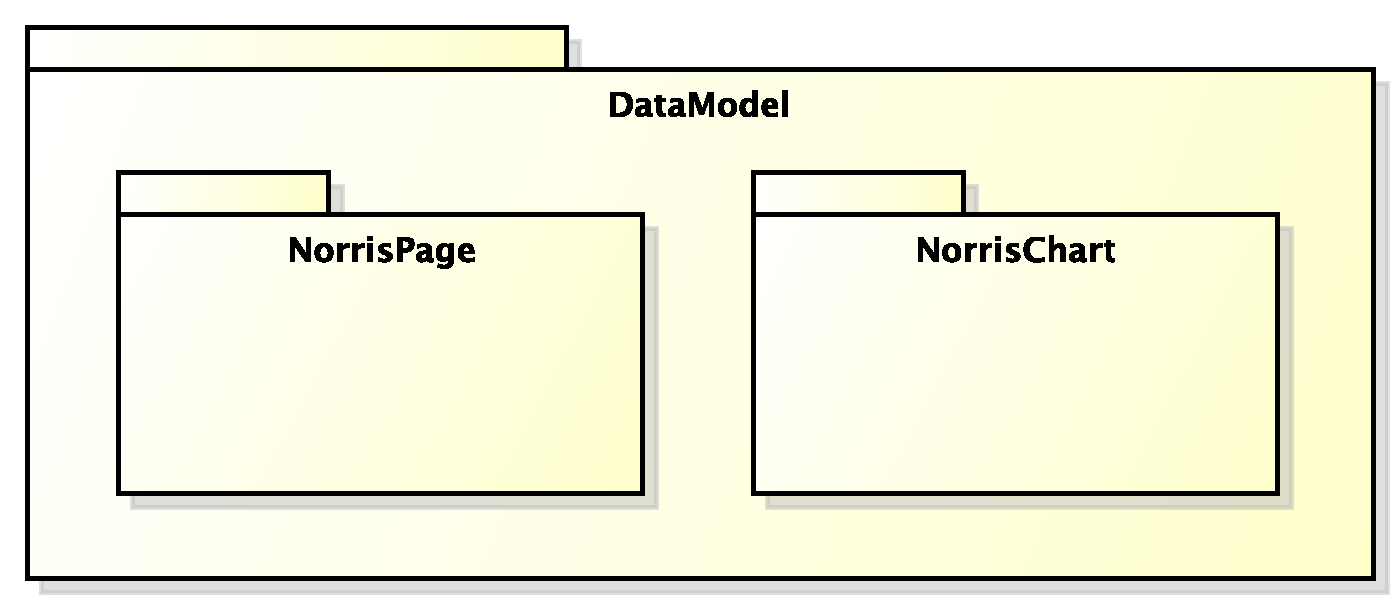
\includegraphics[scale=0.5]{DefinizioneDiProdotto/Pics/Classi/Norris--DataModel}
				\caption{Norris::DataModel}
			\end{figure}
		}
	

			\begin{itemize}
			\item \textbf{Nome:} DataModel
			\item \textbf{Tipo:} package
			
			\item \textbf{Descrizione:} DataModel è il package che astrae un’istanza di Norris. Al suo interno vi sono le informazioni relative alla struttura di grafici e pagine, assieme alle rispettive impostazioni. Inoltre vengono fissate le regole con le quali grafici e pagine vengono composti assieme per formare un’istanza di Norris. Il DataModel fornisce i metodi per inserire i dati e configurare le impostazioni. Fornisce inoltre dei metodi per ottenere i valori di queste ultime, in modo da poterle riutilizzare per un altro grafico o pagina. Infine sono presenti le classi che permettono che vengano memorizzate le informazioni inerenti l’autenticazione.

			\end{itemize}

			
			\level{4}[NorrisChart]{Norris::DataModel::NorrisChart}
			

		\IfFileExists{DefinizioneDiProdotto/Pics/Classi/Norris--DataModel--NorrisChart.pdf}{
			\begin{figure}[H]
				\centering
				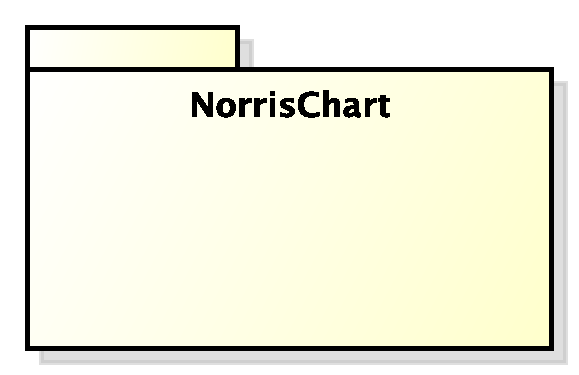
\includegraphics[scale=0.5]{DefinizioneDiProdotto/Pics/Classi/Norris--DataModel--NorrisChart}
				\caption{Norris::DataModel::NorrisChart}
			\end{figure}
		}
	

			\begin{itemize}
			\item \textbf{Nome:} NorrisChart
			\item \textbf{Tipo:} package
			
			\item \textbf{Descrizione:} NorrisChart è il package, le cui classi contengono i dati riguardanti i grafici con le relative impostazioni. Contiene le classi per ogni tipo di grafico, nelle quali sono implementati i metodi, per inserire i dati e configurare le impostazioni, e per ottenere tali valori. Inoltre, le classi di questo package mettono a disposizione le modalità di aggiornamento dei grafici.
			\end{itemize}

			
			\level{5}[BarChartImpl]{Norris::DataModel::NorrisChart::BarChartImpl}
			

		\IfFileExists{DefinizioneDiProdotto/Pics/Classi/Norris--DataModel--NorrisChart--BarChartImpl.pdf}{
			\begin{figure}[H]
				\centering
				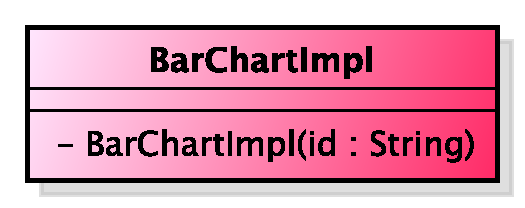
\includegraphics[scale=0.5]{DefinizioneDiProdotto/Pics/Classi/Norris--DataModel--NorrisChart--BarChartImpl}
				\caption{Norris::DataModel::NorrisChart::BarChartImpl}
			\end{figure}
		}
	
			
			\begin{itemize}
			\item \textbf{Nome:} BarChartImpl
			\item \textbf{Tipo:} classe
			
		\item \textbf{Estende:}
		ChartImpl
		\item \textbf{Astratta:}
		no
			\item \textbf{Visibilità:} package
			\item \textbf{Descrizione:} Questa classe rappresenta un grafico di tipo bar chart. Essa contiene al suo interno i dati (BarChartDataObject) e le impostazioni (BarChartSettingsObject) relativi al grafico. Inoltre contiene la classe BarChartInPlaceUpdater, la quale implementa l'aggiornamento di tipo in place per il grafico in questione. Un'istanza della classe BarChartImpl viene creata dalla classe factory BarChartFactory.

			\item \textbf{Metodi:}
				\begin{itemize}
				\setlength{\itemsep}{5pt}
				
					\item[\ding{111}] {{--BarChartImpl(id : String)}} \\ [1mm] Questo metodo è il costruttore della classe. Esso è privato perchè non può esser creata una istanza se non dalla sua classe interna factory.
				\end{itemize}
		
			\end{itemize}

			
			\level{5}[BarChartFactory]{Norris::DataModel::NorrisChart::BarChartImpl::BarChartFactory}
			

		\IfFileExists{DefinizioneDiProdotto/Pics/Classi/Norris--DataModel--NorrisChart--BarChartImpl--BarChartFactory.pdf}{
			\begin{figure}[H]
				\centering
				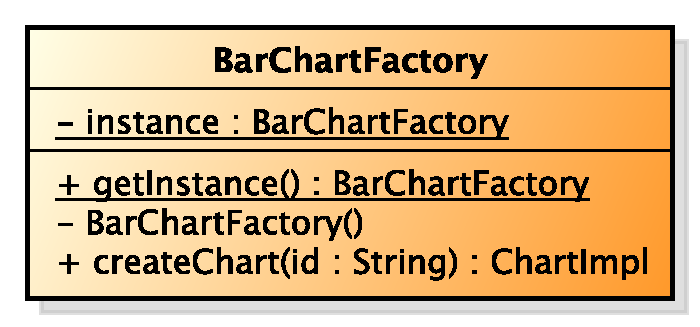
\includegraphics[scale=0.5]{DefinizioneDiProdotto/Pics/Classi/Norris--DataModel--NorrisChart--BarChartImpl--BarChartFactory}
				\caption{Norris::DataModel::NorrisChart::BarChartImpl::BarChartFactory}
			\end{figure}
		}
	
			
			\begin{itemize}
			\item \textbf{Nome:} BarChartFactory
			\item \textbf{Tipo:} classe
			
		\item \textbf{Astratta:}
		no
			\item \textbf{Visibilità:} private
			\item \textbf{Descrizione:} Questa classe si occupa della creazione di un grafico di tipo BarChartImpl. In particolare si occupa di configurare i dati e le impostazioni del grafico. Tale classe dispone di un blocco di inizializzazione statica che registra la sua istanza nel HashMap factories della classe ChartImpl non appena tale classe viene caricata.
			\item \textbf{Attributi:}
				\begin{itemize}
				\setlength{\itemsep}{5pt}
				
					\item[\ding{111}] \underline{--instance : BarChartFactory} \\ [1mm] Questo attributo è il riferimento all'unica istanza della classe.
				\end{itemize}
		
			\item \textbf{Metodi:}
				\begin{itemize}
				\setlength{\itemsep}{5pt}
				
					\item[\ding{111}] {\underline{+getInstance() : BarChartFactory}} \\ [1mm] Questo metodo permette di ottenere l'unica istanza esistente della classe.
					\item[\ding{111}] {{--BarChartFactory()}} \\ [1mm] Questo metodo è il costruttore della classe. Esso è privato perchè non si vuole permettere a nessuno di poter creare un’istanza se non utilizzando il metodo getInstance().

					\item[\ding{111}] {{+createChart(id : String) : ChartImpl}} \\ [1mm] Tale metodo ha il compito di creare la relativa specializzazione di ChartImpl. Esso può accedere al suo costruttore perchè questa classe factory è interna alla relativa classe BarChartImpl.
				\end{itemize}
		
			\end{itemize}

			
			\level{5}[BarChartInPlaceUpdater]{Norris::DataModel::NorrisChart::BarChartInPlaceUpdater}
			

		\IfFileExists{DefinizioneDiProdotto/Pics/Classi/Norris--DataModel--NorrisChart--BarChartInPlaceUpdater.pdf}{
			\begin{figure}[H]
				\centering
				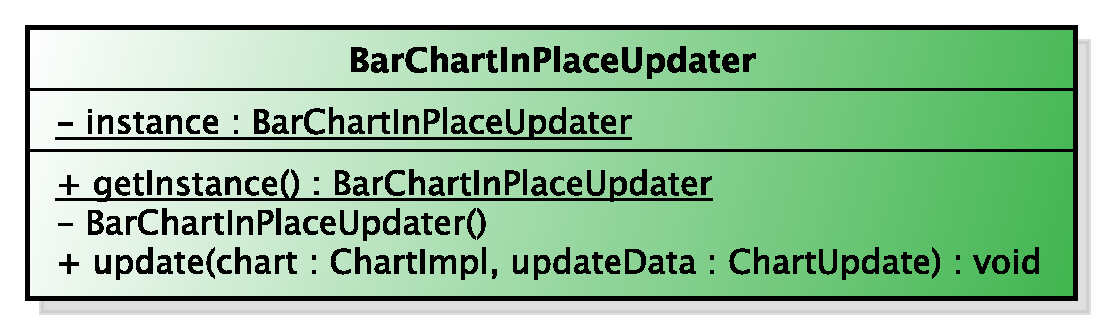
\includegraphics[scale=0.5]{DefinizioneDiProdotto/Pics/Classi/Norris--DataModel--NorrisChart--BarChartInPlaceUpdater}
				\caption{Norris::DataModel::NorrisChart::BarChartInPlaceUpdater}
			\end{figure}
		}
	
			
			\begin{itemize}
			\item \textbf{Nome:} BarChartInPlaceUpdater
			\item \textbf{Tipo:} classe
			
		\item \textbf{Astratta:}
		no
			\item \textbf{Visibilità:} package
			\item \textbf{Descrizione:} Questa classe si occupa di definire il metodo di aggiornamento in place per un grafico di tipo bar chart. In particolare modifica il DataObject contenuto in BarChartImpl tramite il metodo opportuno.
			\item \textbf{Attributi:}
				\begin{itemize}
				\setlength{\itemsep}{5pt}
				
					\item[\ding{111}] \underline{--instance : BarChartInPlaceUpdater} \\ [1mm] Questo attributo è il riferimento all'unica istanza della classe.
				\end{itemize}
		
			\item \textbf{Metodi:}
				\begin{itemize}
				\setlength{\itemsep}{5pt}
				
					\item[\ding{111}] {\underline{+getInstance() : BarChartInPlaceUpdater}} \\ [1mm] Questo metodo permette di ottenere l'unica istanza esistente della classe.
					\item[\ding{111}] {{--BarChartInPlaceUpdater()}} \\ [1mm] Questo metodo è il costruttore della classe.
					\item[\ding{111}] {{+update(chart : ChartImpl, updateData : ChartUpdate) : void}} \\ [1mm] Questo metodo permette di aggiornare il chart passato come primo parametro utilizzando i dati passati come secondo parametro.
				\end{itemize}
		
			\end{itemize}

			
			\level{5}[ChartImpl]{Norris::DataModel::NorrisChart::ChartImpl}
			

		\IfFileExists{DefinizioneDiProdotto/Pics/Classi/Norris--DataModel--NorrisChart--ChartImpl.pdf}{
			\begin{figure}[H]
				\centering
				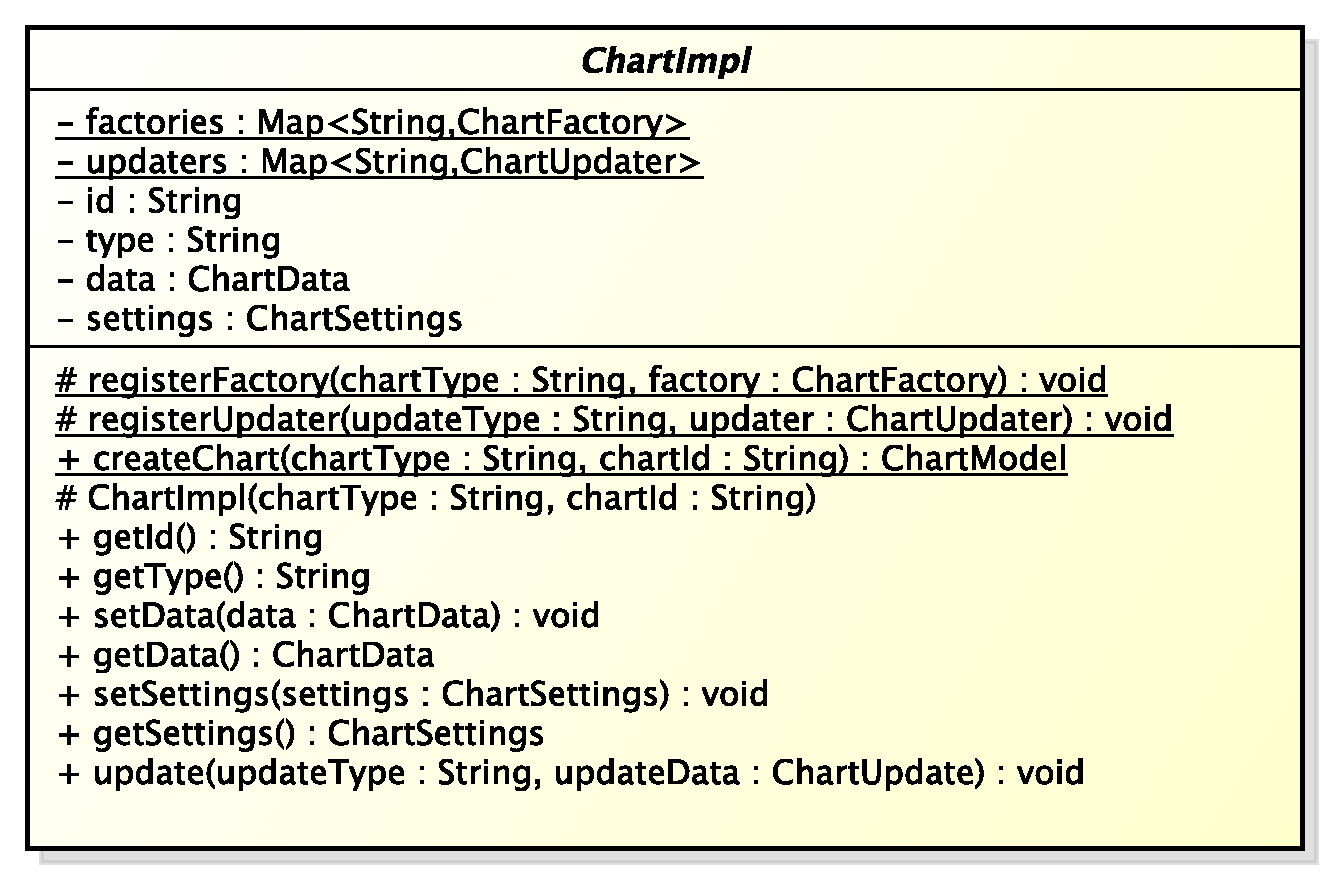
\includegraphics[scale=0.5]{DefinizioneDiProdotto/Pics/Classi/Norris--DataModel--NorrisChart--ChartImpl}
				\caption{Norris::DataModel::NorrisChart::ChartImpl}
			\end{figure}
		}
	
			
			\begin{itemize}
			\item \textbf{Nome:} ChartImpl
			\item \textbf{Tipo:} classe
			
		\item \textbf{Estende:}
		EventEmitter
		\item \textbf{Astratta:}
		si
			\item \textbf{Visibilità:} public
			\item \textbf{Descrizione:} Questa classe rappresenta un grafico generico e per questo motivo è una classe astratta. Essa contiene al suo interno i dati (ChartData) e le impostazioni (ChartSettings) relativi al grafico. Inoltre contiene l' interfaccia ChartFactory. Sono inoltre presenti due hashmap: la prima si occupa della corrispondenza tra le tipologie di grafico e le rispettive classi factory, la seconda invece si occupa della corrispondenza tra le varie tipologie di aggiornamento e la classe che implementa tale aggiornamento per un tipo specifico di grafico. ChartImpl ha una dipendenza verso l'interfaccia ChartUpdate, in quanto deve conoscere il tipo del pacchetto degli aggiornamenti.
			\item \textbf{Attributi:}
				\begin{itemize}
				\setlength{\itemsep}{5pt}
				
					\item[\ding{111}] \underline{--factories : Map<String,ChartFactory>} \\ [1mm] Questo attributo contiene le dipendenze necessarie per istanziare nuovi grafici. La chiave del HashMap rappresenta
					\item[\ding{111}] \underline{--updaters : Map<String,ChartUpdater>} \\ [1mm] Questo attributo contiene le dipendenze necessarie per aggiornare i grafici.
					\item[\ding{111}] {--id : String} \\ [1mm] Questo attributo consiste nell'id del grafico.
					\item[\ding{111}] {--type : String}
					\item[\ding{111}] {--data : ChartData} \\ [1mm] Questo attributo contiene i dati rappresentati dal grafico.
					\item[\ding{111}] {--settings : ChartSettings} \\ [1mm] Questo attributo contiene le impostazioni del grafico.
				\end{itemize}
		
			\item \textbf{Metodi:}
				\begin{itemize}
				\setlength{\itemsep}{5pt}
				
					\item[\ding{111}] {\underline{\#registerFactory(chartType : String, factory : ChartFactory) : void}} \\ [1mm] Tale metodo serve per registrare una certa factory al relativo chart nel HashMap della classe (factories). Tale metodo viene chiamato dalle classi factory interne ai vari ChartImpl con lo scopo di registrarsi come creatori di chart e poter quindi esser utilizzate per tale scopo.
					\item[\ding{111}] {\underline{\#registerUpdater(updateType : String, updater : ChartUpdater) : void}} \\ [1mm] Tale metodo serve per registrare un certo updater al relativo tipo di update nel MashMap della classe (updaters). Tale metodo viene invocato dalle classi Updater al loro caricamento per aggiungersi come updater.
					\item[\ding{111}] {\underline{+createChart(chartType : String, chartId : String) : ChartImpl}} \\ [1mm] Tale metodo non fa altro che creare il chart associato al parametro type e ritornare l’interfaccia ChartModel di tale istanza creata. Esso non fa altro che invocare il metodo chreateChart dela classe factory pesente nel HashMap factories con la chiave eguale al parametro type e ne ritornerà tale oggetto creato.
					\item[\ding{111}] {{\#ChartImpl(chartType : String, chartId : String)}} \\ [1mm] Questo metodo è il costruttore della classe. Esso è accessibile solamente alle sottoclassi per la creazione del sottoggetto.
					\item[\ding{111}] {{+getId() : String}} \\ [1mm] Questo metodo permette di ottenere l'id del grafico.
					\item[\ding{111}] {{+getType() : String}} \\ [1mm] Questo metodo permette di ottenere il tipo del grafico.
					\item[\ding{111}] {{+setData(data : ChartData) : void}} \\ [1mm] Questo metodo permette di impostare i dati del grafico.
					\item[\ding{111}] {{+getData() : ChartData}} \\ [1mm] Questo metodo permette di ottenere i dati del grafico.
					\item[\ding{111}] {{+setSettings(settings : ChartSettings) : void}} \\ [1mm] Questo metodo permette di impostare le opzioni del grafico.
					\item[\ding{111}] {{+getSettings() : ChartSettings}} \\ [1mm] Questo metodo permette di ottenere le opzioni del grafico.
					\item[\ding{111}] {{+update(updateType : String, updateData : ChartUpdate) : void}} \\ [1mm] Tale metodo ha il compito di aggiornare i chart utilizzando la tipologia di aggiornamento presente in updateType e il pacchetto di aggiornamento updateData. Esso non fa altro che invocare il metodo update dell’updater pesente nel HashMap updaters con la chiave eguale al parametro updateType e passargli come parametro il parametro ricevuto updateData ed i dati del chart che verranno modificati per riferimento.
				\end{itemize}
		
			\end{itemize}

			
			\level{5}[LineChartImpl]{Norris::DataModel::NorrisChart::LineChartImpl}
			

		\IfFileExists{DefinizioneDiProdotto/Pics/Classi/Norris--DataModel--NorrisChart--LineChartImpl.pdf}{
			\begin{figure}[H]
				\centering
				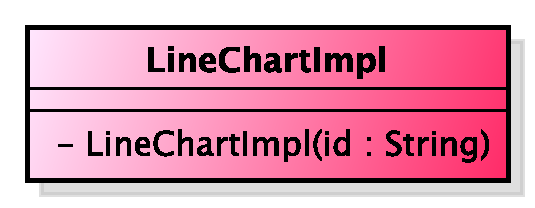
\includegraphics[scale=0.5]{DefinizioneDiProdotto/Pics/Classi/Norris--DataModel--NorrisChart--LineChartImpl}
				\caption{Norris::DataModel::NorrisChart::LineChartImpl}
			\end{figure}
		}
	
			
			\begin{itemize}
			\item \textbf{Nome:} LineChartImpl
			\item \textbf{Tipo:} classe
			
		\item \textbf{Estende:}
		ChartImpl
		\item \textbf{Astratta:}
		no
			\item \textbf{Visibilità:} package
			\item \textbf{Descrizione:} Questa classe rappresenta un grafico di tipo line chart. Essa contiene al suo interno i dati (LineChartDataObject) e le impostazioni (LineChartSettingsObject) relativi al grafico. Inoltre contiene le classi LineChartInPlaceUpdater e LineChartStreamUpdater, le quali implementano rispettivamente l'aggiornamento di tipo in place e stream per il grafico in questione. Un'istanza della classe LineChartImpl viene creata dalla classe factory LineChartFactory.
			\item \textbf{Metodi:}
				\begin{itemize}
				\setlength{\itemsep}{5pt}
				
					\item[\ding{111}] {{--LineChartImpl(id : String)}} \\ [1mm] Questo metodo è il costruttore della classe. Esso è privato perchè non può esser creata una istanza se non dalla sua classe interna factory.
				\end{itemize}
		
			\end{itemize}

			
			\level{5}[LineChartFactory]{Norris::DataModel::NorrisChart::LineChartImpl::LineChartFactory}
			

		\IfFileExists{DefinizioneDiProdotto/Pics/Classi/Norris--DataModel--NorrisChart--LineChartImpl--LineChartFactory.pdf}{
			\begin{figure}[H]
				\centering
				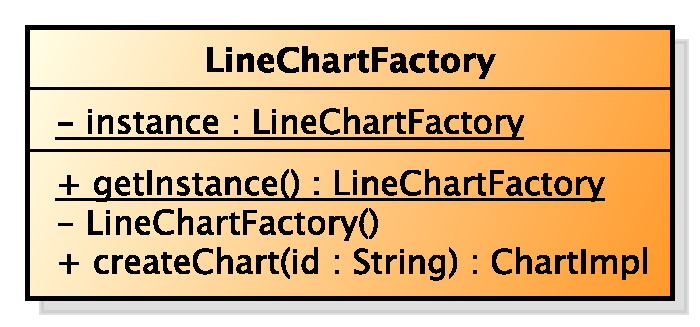
\includegraphics[scale=0.5]{DefinizioneDiProdotto/Pics/Classi/Norris--DataModel--NorrisChart--LineChartImpl--LineChartFactory}
				\caption{Norris::DataModel::NorrisChart::LineChartImpl::LineChartFactory}
			\end{figure}
		}
	
			
			\begin{itemize}
			\item \textbf{Nome:} LineChartFactory
			\item \textbf{Tipo:} classe
			
		\item \textbf{Astratta:}
		no
			\item \textbf{Visibilità:} private
			\item \textbf{Descrizione:} Questa classe si occupa della creazione di un grafico di tipo LineChartImpl. In particolare si occupa di configurare i dati e le impostazioni del grafico. Tale classe dispone di un blocco di inizializzazione statica che registra la sua istanza nel HashMap factories della classe ChartImpl non appena tale classe viene caricata.
			\item \textbf{Attributi:}
				\begin{itemize}
				\setlength{\itemsep}{5pt}
				
					\item[\ding{111}] \underline{--instance : LineChartFactory} \\ [1mm] Questo attributo è il riferimento all'unica istanza della classe.
				\end{itemize}
		
			\item \textbf{Metodi:}
				\begin{itemize}
				\setlength{\itemsep}{5pt}
				
					\item[\ding{111}] {\underline{+getInstance() : LineChartFactory}} \\ [1mm] Questo metodo permette di ottenere l'unica istanza esistente della classe.
					\item[\ding{111}] {{--LineChartFactory()}} \\ [1mm] Questo metodo è il costruttore della classe. Esso è privato perchè non si vuole permettere a nessuno di poter creare un’istanza se non utilizzando il metodo getInstance().

					\item[\ding{111}] {{+createChart(id : String) : ChartImpl}} \\ [1mm] Tale metodo ha il compito di creare la relativa specializzazione di ChartImpl. Esso può accedere al suo costruttore perchè questa classe factory è interna alla relativa classe BarChartImpl.
				\end{itemize}
		
			\end{itemize}

			
			\level{5}[LineChartInPlaceUpdater]{Norris::DataModel::NorrisChart::LineChartInPlaceUpdater}
			

		\IfFileExists{DefinizioneDiProdotto/Pics/Classi/Norris--DataModel--NorrisChart--LineChartInPlaceUpdater.pdf}{
			\begin{figure}[H]
				\centering
				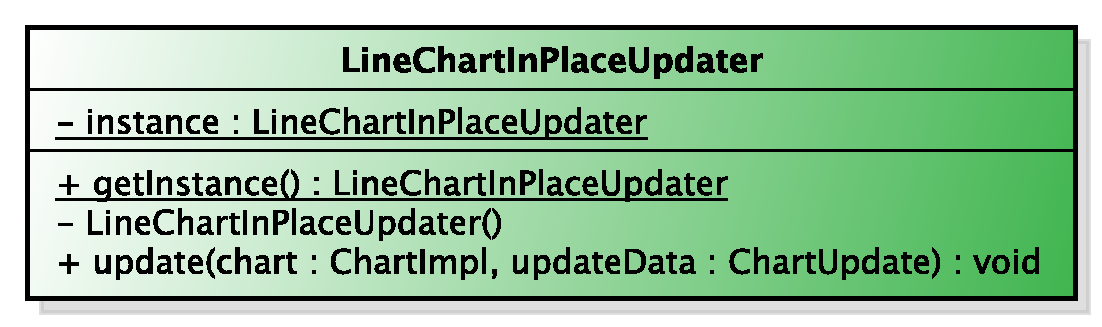
\includegraphics[scale=0.5]{DefinizioneDiProdotto/Pics/Classi/Norris--DataModel--NorrisChart--LineChartInPlaceUpdater}
				\caption{Norris::DataModel::NorrisChart::LineChartInPlaceUpdater}
			\end{figure}
		}
	
			
			\begin{itemize}
			\item \textbf{Nome:} LineChartInPlaceUpdater
			\item \textbf{Tipo:} classe
			
		\item \textbf{Astratta:}
		no
			\item \textbf{Visibilità:} package
			\item \textbf{Descrizione:} Questa classe si occupa di definire il metodo di aggiornamento in place per un grafico di tipo line chart. In particolare modifica il DataObject contenuto in LineChartImpl tramite il metodo opportuno.
			\item \textbf{Attributi:}
				\begin{itemize}
				\setlength{\itemsep}{5pt}
				
					\item[\ding{111}] \underline{--instance : LineChartInPlaceUpdater} \\ [1mm] Questo attributo è il riferimento all'unica istanza della classe.
				\end{itemize}
		
			\item \textbf{Metodi:}
				\begin{itemize}
				\setlength{\itemsep}{5pt}
				
					\item[\ding{111}] {\underline{+getInstance() : LineChartInPlaceUpdater}} \\ [1mm] Questo metodo permette di ottenere l'unica istanza esistente della classe.
					\item[\ding{111}] {{--LineChartInPlaceUpdater()}} \\ [1mm] Questo metodo è il costruttore della classe.
					\item[\ding{111}] {{+update(chart : ChartImpl, updateData : ChartUpdate) : void}} \\ [1mm] Questo metodo permette di aggiornare il chart passato come primo parametro utilizzando i dati passati come secondo parametro.
				\end{itemize}
		
			\end{itemize}

			
			\level{5}[LineChartStreamUpdater]{Norris::DataModel::NorrisChart::LineChartStreamUpdater}
			

		\IfFileExists{DefinizioneDiProdotto/Pics/Classi/Norris--DataModel--NorrisChart--LineChartStreamUpdater.pdf}{
			\begin{figure}[H]
				\centering
				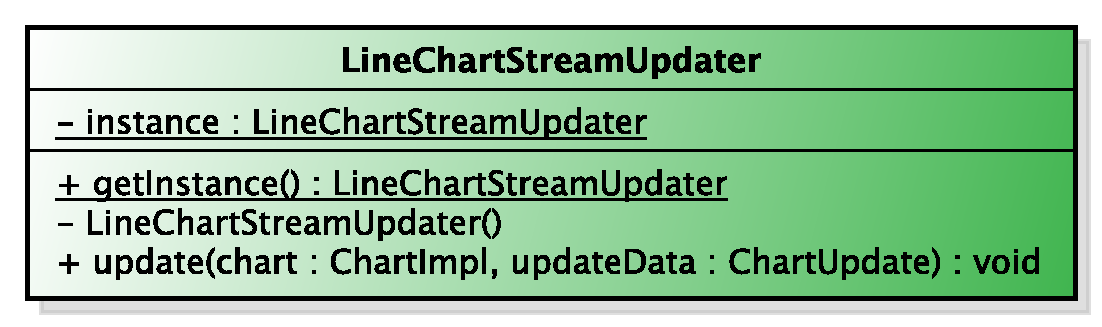
\includegraphics[scale=0.5]{DefinizioneDiProdotto/Pics/Classi/Norris--DataModel--NorrisChart--LineChartStreamUpdater}
				\caption{Norris::DataModel::NorrisChart::LineChartStreamUpdater}
			\end{figure}
		}
	
			
			\begin{itemize}
			\item \textbf{Nome:} LineChartStreamUpdater
			\item \textbf{Tipo:} classe
			
		\item \textbf{Astratta:}
		no
			\item \textbf{Visibilità:} package
			\item \textbf{Descrizione:} Questa classe si occupa di definire il metodo di aggiornamento stream per un grafico di tipo line chart. In particolare modifica il DataObject contenuto in LineChartImpl tramite il metodo opportuno.
			\item \textbf{Attributi:}
				\begin{itemize}
				\setlength{\itemsep}{5pt}
				
					\item[\ding{111}] \underline{--instance : LineChartStreamUpdater} \\ [1mm] Questo attributo è il riferimento all'unica istanza della classe.
				\end{itemize}
		
			\item \textbf{Metodi:}
				\begin{itemize}
				\setlength{\itemsep}{5pt}
				
					\item[\ding{111}] {\underline{+getInstance() : LineChartStreamUpdater}} \\ [1mm] Questo metodo permette di ottenere l'unica istanza esistente della classe.
					\item[\ding{111}] {{--LineChartStreamUpdater()}} \\ [1mm] Questo metodo è il costruttore della classe.
					\item[\ding{111}] {{+update(chart : ChartImpl, updateData : ChartUpdate) : void}} \\ [1mm] Questo metodo permette di aggiornare il chart passato come primo parametro utilizzando i dati passati come secondo parametro.
				\end{itemize}
		
			\end{itemize}

			
			\level{5}[MapChartImpl]{Norris::DataModel::NorrisChart::MapChartImpl}
			

		\IfFileExists{DefinizioneDiProdotto/Pics/Classi/Norris--DataModel--NorrisChart--MapChartImpl.pdf}{
			\begin{figure}[H]
				\centering
				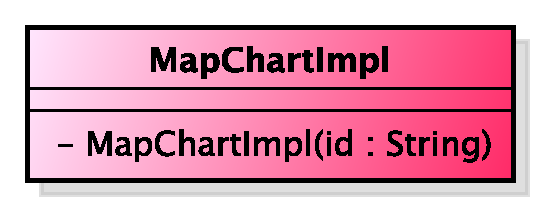
\includegraphics[scale=0.5]{DefinizioneDiProdotto/Pics/Classi/Norris--DataModel--NorrisChart--MapChartImpl}
				\caption{Norris::DataModel::NorrisChart::MapChartImpl}
			\end{figure}
		}
	
			
			\begin{itemize}
			\item \textbf{Nome:} MapChartImpl
			\item \textbf{Tipo:} classe
			
		\item \textbf{Estende:}
		ChartImpl
		\item \textbf{Astratta:}
		no
			\item \textbf{Visibilità:} package
			\item \textbf{Descrizione:} Questa classe rappresenta un grafico di tipo map chart. Essa contiene al suo interno i dati (MapChartDataObject) e le impostazioni (MapChartSettingsObject) relativi al grafico. Inoltre contiene le classi MapChartInPlaceUpdater e MapChartMovieUpdater, le quali implementano rispettivamente l'aggiornamento di tipo in place e movie per il grafico in questione. Un'istanza della classe MapChartImpl viene creata dalla classe factory MapChartFactory.
			\item \textbf{Metodi:}
				\begin{itemize}
				\setlength{\itemsep}{5pt}
				
					\item[\ding{111}] {{--MapChartImpl(id : String)}} \\ [1mm] Questo metodo è il costruttore della classe. Esso è privato perchè non può esser creata una istanza se non dalla sua classe interna factory.
				\end{itemize}
		
			\end{itemize}

			
			\level{5}[MapChartFactory]{Norris::DataModel::NorrisChart::MapChartImpl::MapChartFactory}
			

		\IfFileExists{DefinizioneDiProdotto/Pics/Classi/Norris--DataModel--NorrisChart--MapChartImpl--MapChartFactory.pdf}{
			\begin{figure}[H]
				\centering
				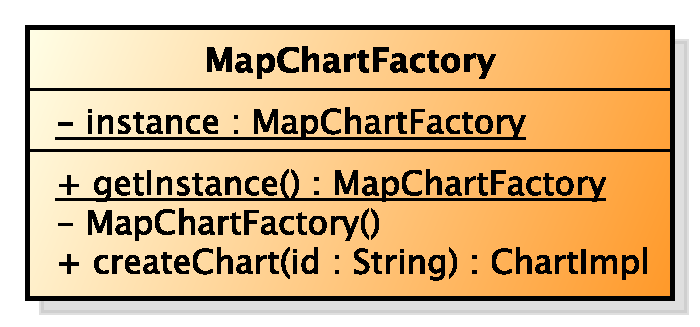
\includegraphics[scale=0.5]{DefinizioneDiProdotto/Pics/Classi/Norris--DataModel--NorrisChart--MapChartImpl--MapChartFactory}
				\caption{Norris::DataModel::NorrisChart::MapChartImpl::MapChartFactory}
			\end{figure}
		}
	
			
			\begin{itemize}
			\item \textbf{Nome:} MapChartFactory
			\item \textbf{Tipo:} classe
			
		\item \textbf{Astratta:}
		no
			\item \textbf{Visibilità:} private
			\item \textbf{Descrizione:} Questa classe si occupa della creazione di un grafico di tipo MapChartImpl. In particolare si occupa di configurare i dati e le impostazioni del grafico. Tale classe dispone di un blocco di inizializzazione statica che registra la sua istanza nel HashMap factories della classe ChartImpl non appena tale classe viene caricata.
			\item \textbf{Attributi:}
				\begin{itemize}
				\setlength{\itemsep}{5pt}
				
					\item[\ding{111}] \underline{--instance : MapChartFactory} \\ [1mm] Questo attributo è il riferimento all'unica istanza della classe.
				\end{itemize}
		
			\item \textbf{Metodi:}
				\begin{itemize}
				\setlength{\itemsep}{5pt}
				
					\item[\ding{111}] {\underline{+getInstance() : MapChartFactory}} \\ [1mm] Questo metodo permette di ottenere l'unica istanza esistente della classe.
					\item[\ding{111}] {{--MapChartFactory()}} \\ [1mm] Questo metodo è il costruttore della classe. Esso è privato perchè non si vuole permettere a nessuno di poter creare un’istanza se non utilizzando il metodo getInstance().

					\item[\ding{111}] {{+createChart(id : String) : ChartImpl}} \\ [1mm] Tale metodo ha il compito di creare la relativa specializzazione di ChartImpl. Esso può accedere al suo costruttore perchè questa classe factory è interna alla relativa classe BarChartImpl.
				\end{itemize}
		
			\end{itemize}

			
			\level{5}[MapChartInPlaceUpdater]{Norris::DataModel::NorrisChart::MapChartInPlaceUpdater}
			

		\IfFileExists{DefinizioneDiProdotto/Pics/Classi/Norris--DataModel--NorrisChart--MapChartInPlaceUpdater.pdf}{
			\begin{figure}[H]
				\centering
				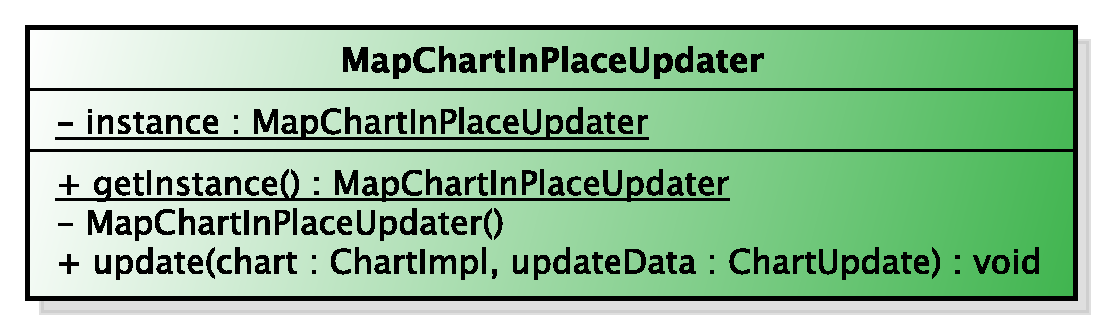
\includegraphics[scale=0.5]{DefinizioneDiProdotto/Pics/Classi/Norris--DataModel--NorrisChart--MapChartInPlaceUpdater}
				\caption{Norris::DataModel::NorrisChart::MapChartInPlaceUpdater}
			\end{figure}
		}
	
			
			\begin{itemize}
			\item \textbf{Nome:} MapChartInPlaceUpdater
			\item \textbf{Tipo:} classe
			
		\item \textbf{Astratta:}
		no
			\item \textbf{Visibilità:} package
			\item \textbf{Descrizione:} Questa classe si occupa di definire il metodo di aggiornamento in place per un grafico di tipo map chart. In particolare modifica il DataObject contenuto in MapChartImpl tramite il metodo opportuno.
			\item \textbf{Attributi:}
				\begin{itemize}
				\setlength{\itemsep}{5pt}
				
					\item[\ding{111}] \underline{--instance : MapChartInPlaceUpdater} \\ [1mm] Questo attributo è il riferimento all'unica istanza della classe.
				\end{itemize}
		
			\item \textbf{Metodi:}
				\begin{itemize}
				\setlength{\itemsep}{5pt}
				
					\item[\ding{111}] {\underline{+getInstance() : MapChartInPlaceUpdater}} \\ [1mm] Questo metodo permette di ottenere l'unica istanza esistente della classe.
					\item[\ding{111}] {{--MapChartInPlaceUpdater()}} \\ [1mm] Questo metodo è il costruttore della classe.
					\item[\ding{111}] {{+update(chart : ChartImpl, updateData : ChartUpdate) : void}} \\ [1mm] Questo metodo permette di aggiornare il chart passato come primo parametro utilizzando i dati passati come secondo parametro.
				\end{itemize}
		
			\end{itemize}

			
			\level{5}[MapChartMovieUpdater]{Norris::DataModel::NorrisChart::MapChartMovieUpdater}
			

		\IfFileExists{DefinizioneDiProdotto/Pics/Classi/Norris--DataModel--NorrisChart--MapChartMovieUpdater.pdf}{
			\begin{figure}[H]
				\centering
				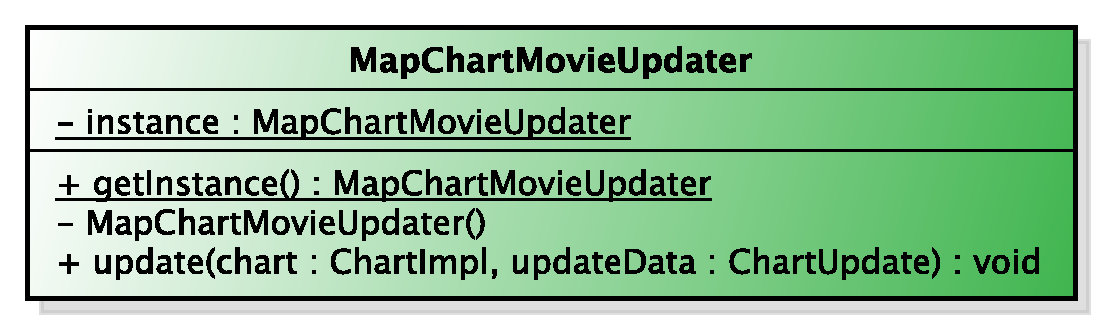
\includegraphics[scale=0.5]{DefinizioneDiProdotto/Pics/Classi/Norris--DataModel--NorrisChart--MapChartMovieUpdater}
				\caption{Norris::DataModel::NorrisChart::MapChartMovieUpdater}
			\end{figure}
		}
	
			
			\begin{itemize}
			\item \textbf{Nome:} MapChartMovieUpdater
			\item \textbf{Tipo:} classe
			
		\item \textbf{Astratta:}
		no
			\item \textbf{Visibilità:} package
			\item \textbf{Descrizione:} Questa classe si occupa di definire il metodo di aggiornamento movie per un grafico di tipo map chart. In particolare modifica il DataObject contenuto in MapChartImpl tramite il metodo opportuno.
			\item \textbf{Attributi:}
				\begin{itemize}
				\setlength{\itemsep}{5pt}
				
					\item[\ding{111}] \underline{--instance : MapChartMovieUpdater} \\ [1mm] Questo attributo è il riferimento all'unica istanza della classe.
				\end{itemize}
		
			\item \textbf{Metodi:}
				\begin{itemize}
				\setlength{\itemsep}{5pt}
				
					\item[\ding{111}] {\underline{+getInstance() : MapChartMovieUpdater}} \\ [1mm] Questo metodo permette di ottenere l'unica istanza esistente della classe.
					\item[\ding{111}] {{--MapChartMovieUpdater()}} \\ [1mm] Questo metodo è il costruttore della classe.
					\item[\ding{111}] {{+update(chart : ChartImpl, updateData : ChartUpdate) : void}} \\ [1mm] Questo metodo permette di aggiornare il chart passato come primo parametro utilizzando i dati passati come secondo parametro.
				\end{itemize}
		
			\end{itemize}

			
			\level{5}[TableImpl]{Norris::DataModel::NorrisChart::TableImpl}
			

		\IfFileExists{DefinizioneDiProdotto/Pics/Classi/Norris--DataModel--NorrisChart--TableImpl.pdf}{
			\begin{figure}[H]
				\centering
				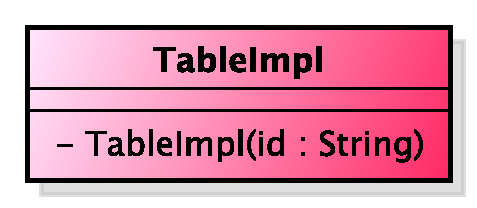
\includegraphics[scale=0.5]{DefinizioneDiProdotto/Pics/Classi/Norris--DataModel--NorrisChart--TableImpl}
				\caption{Norris::DataModel::NorrisChart::TableImpl}
			\end{figure}
		}
	
			
			\begin{itemize}
			\item \textbf{Nome:} TableImpl
			\item \textbf{Tipo:} classe
			
		\item \textbf{Estende:}
		ChartImpl
		\item \textbf{Astratta:}
		no
			\item \textbf{Visibilità:} package
			\item \textbf{Descrizione:} Questa classe rappresenta un grafico di tipo table. Essa contiene al suo interno i dati (TableDataObject) e le impostazioni (TableSettingsObject) relativi al grafico. Inoltre contiene le classi TableInPlaceUpdater e TableStreamUpdater, le quali implementano rispettivamente l'aggiornamento di tipo in place e stream per il grafico in questione. Un'istanza della classe TableImpl viene creata dalla classe factory TableFactory.
			\item \textbf{Metodi:}
				\begin{itemize}
				\setlength{\itemsep}{5pt}
				
					\item[\ding{111}] {{--TableImpl(id : String)}} \\ [1mm] Questo metodo è il costruttore della classe. Esso è privato perchè non può esser creata una istanza se non dalla sua classe interna factory.
				\end{itemize}
		
			\end{itemize}

			
			\level{5}[TableFactory]{Norris::DataModel::NorrisChart::TableImpl::TableFactory}
			

		\IfFileExists{DefinizioneDiProdotto/Pics/Classi/Norris--DataModel--NorrisChart--TableImpl--TableFactory.pdf}{
			\begin{figure}[H]
				\centering
				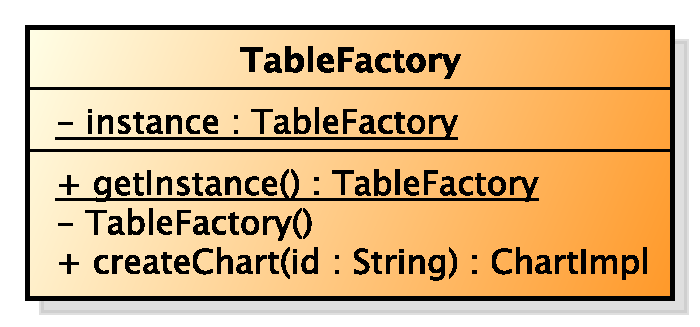
\includegraphics[scale=0.5]{DefinizioneDiProdotto/Pics/Classi/Norris--DataModel--NorrisChart--TableImpl--TableFactory}
				\caption{Norris::DataModel::NorrisChart::TableImpl::TableFactory}
			\end{figure}
		}
	
			
			\begin{itemize}
			\item \textbf{Nome:} TableFactory
			\item \textbf{Tipo:} classe
			
		\item \textbf{Astratta:}
		no
			\item \textbf{Visibilità:} private
			\item \textbf{Descrizione:} Questa classe si occupa della creazione di un grafico di tipo TableImpl. In particolare si occupa di configurare i dati e le impostazioni del grafico. Tale classe dispone di un blocco di inizializzazione statica che registra la sua istanza nel HashMap factories della classe ChartImpl non appena tale classe viene caricata.
			\item \textbf{Attributi:}
				\begin{itemize}
				\setlength{\itemsep}{5pt}
				
					\item[\ding{111}] \underline{--instance : TableFactory} \\ [1mm] Questo attributo è il riferimento all'unica istanza della classe.
				\end{itemize}
		
			\item \textbf{Metodi:}
				\begin{itemize}
				\setlength{\itemsep}{5pt}
				
					\item[\ding{111}] {\underline{+getInstance() : TableFactory}} \\ [1mm] Questo metodo permette di ottenere l'unica istanza esistente della classe.
					\item[\ding{111}] {{--TableFactory()}} \\ [1mm] Questo metodo è il costruttore della classe. Esso è privato perchè non si vuole permettere a nessuno di poter creare un’istanza se non utilizzando il metodo getInstance().
					\item[\ding{111}] {{+createChart(id : String) : ChartImpl}} \\ [1mm] Tale metodo ha il compito di creare la relativa specializzazione di ChartImpl. Esso può accedere al suo costruttore perchè questa classe factory è interna alla relativa classe BarChartImpl.
				\end{itemize}
		
			\end{itemize}

			
			\level{5}[TableInPlaceUpdater]{Norris::DataModel::NorrisChart::TableInPlaceUpdater}
			

		\IfFileExists{DefinizioneDiProdotto/Pics/Classi/Norris--DataModel--NorrisChart--TableInPlaceUpdater.pdf}{
			\begin{figure}[H]
				\centering
				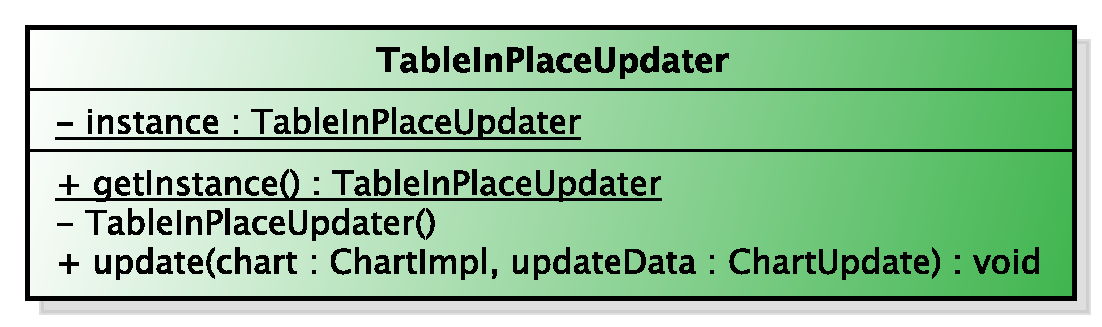
\includegraphics[scale=0.5]{DefinizioneDiProdotto/Pics/Classi/Norris--DataModel--NorrisChart--TableInPlaceUpdater}
				\caption{Norris::DataModel::NorrisChart::TableInPlaceUpdater}
			\end{figure}
		}
	
			
			\begin{itemize}
			\item \textbf{Nome:} TableInPlaceUpdater
			\item \textbf{Tipo:} classe
			
		\item \textbf{Astratta:}
		no
			\item \textbf{Visibilità:} package
			\item \textbf{Descrizione:} Questa classe si occupa di definire il metodo di aggiornamento in place per un grafico di tipo table. In particolare modifica il DataObject contenuto in Table tramite il metodo opportuno.
			\item \textbf{Attributi:}
				\begin{itemize}
				\setlength{\itemsep}{5pt}
				
					\item[\ding{111}] \underline{--instance : TableInPlaceUpdater} \\ [1mm] Questo attributo è il riferimento all'unica istanza della classe.
				\end{itemize}
		
			\item \textbf{Metodi:}
				\begin{itemize}
				\setlength{\itemsep}{5pt}
				
					\item[\ding{111}] {\underline{+getInstance() : TableInPlaceUpdater}} \\ [1mm] Questo metodo permette di ottenere l'unica istanza esistente della classe.
					\item[\ding{111}] {{--TableInPlaceUpdater()}} \\ [1mm] Questo metodo permette di aggiornare il chart passato come primo parametro utilizzando i dati passati come secondo parametro.
					\item[\ding{111}] {{+update(chart : ChartImpl, updateData : ChartUpdate) : void}} \\ [1mm] Questo metodo permette di aggiornare il chart passato come primo parametro utilizzando i dati passati come secondo parametro.
				\end{itemize}
		
			\end{itemize}

			
			\level{5}[TableStreamUpdater]{Norris::DataModel::NorrisChart::TableStreamUpdater}
			

		\IfFileExists{DefinizioneDiProdotto/Pics/Classi/Norris--DataModel--NorrisChart--TableStreamUpdater.pdf}{
			\begin{figure}[H]
				\centering
				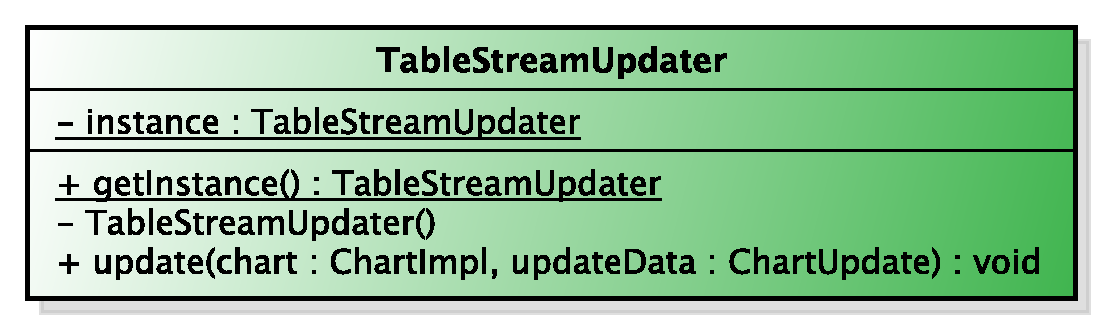
\includegraphics[scale=0.5]{DefinizioneDiProdotto/Pics/Classi/Norris--DataModel--NorrisChart--TableStreamUpdater}
				\caption{Norris::DataModel::NorrisChart::TableStreamUpdater}
			\end{figure}
		}
	
			
			\begin{itemize}
			\item \textbf{Nome:} TableStreamUpdater
			\item \textbf{Tipo:} classe
			
		\item \textbf{Astratta:}
		no
			\item \textbf{Visibilità:} package
			\item \textbf{Descrizione:} Questa classe si occupa di definire il metodo di aggiornamento stream per un grafico di tipo table. In particolare modifica il DataObject contenuto in Table tramite il metodo opportuno.
			\item \textbf{Attributi:}
				\begin{itemize}
				\setlength{\itemsep}{5pt}
				
					\item[\ding{111}] \underline{--instance : TableStreamUpdater} \\ [1mm] Questo attributo è il riferimento all'unica istanza della classe.
				\end{itemize}
		
			\item \textbf{Metodi:}
				\begin{itemize}
				\setlength{\itemsep}{5pt}
				
					\item[\ding{111}] {\underline{+getInstance() : TableStreamUpdater}} \\ [1mm] Questo metodo permette di ottenere l'unica istanza esistente della classe.
					\item[\ding{111}] {{--TableStreamUpdater()}} \\ [1mm] Questo metodo è il costruttore della classe.
					\item[\ding{111}] {{+update(chart : ChartImpl, updateData : ChartUpdate) : void}} \\ [1mm] Questo metodo permette di aggiornare il chart passato come primo parametro utilizzando i dati passati come secondo parametro.
				\end{itemize}
		
			\end{itemize}

			
			\level{5}[NorrisImpl]{Norris::DataModel::NorrisImpl}
			

		\IfFileExists{DefinizioneDiProdotto/Pics/Classi/Norris--DataModel--NorrisImpl.pdf}{
			\begin{figure}[H]
				\centering
				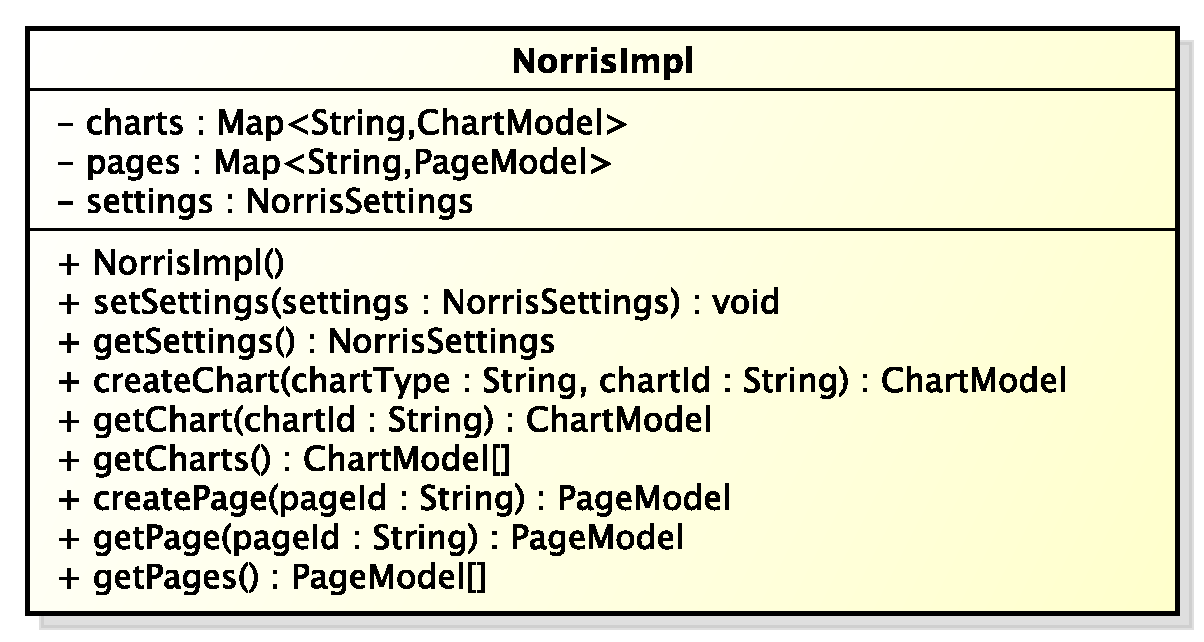
\includegraphics[scale=0.5]{DefinizioneDiProdotto/Pics/Classi/Norris--DataModel--NorrisImpl}
				\caption{Norris::DataModel::NorrisImpl}
			\end{figure}
		}
	
			
			\begin{itemize}
			\item \textbf{Nome:} NorrisImpl
			\item \textbf{Tipo:} classe
			
		\item \textbf{Estende:}
		EventEmitter
		\item \textbf{Astratta:}
		no
			\item \textbf{Visibilità:} public
			\item \textbf{Descrizione:} NorrisImpl implementa l'interfaccia NorrisModel e rappresenta il modello di un'istanza di Norris. Essa contiene al suo interno dei grafici (ChartImpl), delle pagine (PageImpl) e le impostazioni relative all'istanza di Norris. Tra queste ci sono le funzioni di autenticazione.
			\item \textbf{Attributi:}
				\begin{itemize}
				\setlength{\itemsep}{5pt}
				
					\item[\ding{111}] {--charts : Map<String,ChartImpl>} \\ [1mm] Questo attributo consiste nell'insieme dei grafici presenti nell'istanza di Norris.
					\item[\ding{111}] {--pages : Map<String,PageImpl>}
					\item[\ding{111}] {--settings : NorrisSettings} \\ [1mm] Questo attributo consiste nelle opzioni dell'istanza di Norris.
				\end{itemize}
		
			\item \textbf{Metodi:}
				\begin{itemize}
				\setlength{\itemsep}{5pt}
				
					\item[\ding{111}] {{+NorrisImpl(settings : NorrisSettings)}} \\ [1mm] Questo metodo è il costruttore della classe.
					\item[\ding{111}] {{+getSettings() : NorrisSettings}} \\ [1mm] Questo metodo permette di ottenere le impostazioni relative all'istanza di Norris.
					\item[\ding{111}] {{+createChart(chartType : String, chartId : String) : ChartImpl}} \\ [1mm] Questo metodo permette di creare un nuovo grafico e di aggiungerlo all'istanza di Norris.
					\item[\ding{111}] {{+getChart(chartId : String) : ChartImpl}} \\ [1mm] Questo metodo permette di ottenere un grafico presente nell'istanza di Norris dato il suo id.
					\item[\ding{111}] {{+getCharts() : ChartImpl}} \\ [1mm] Questo metodo permette di ottenere tutti i grafici presenti nell'istanza di Norris.
					\item[\ding{111}] {{+createPage(pageId : String) : PageImpl}} \\ [1mm] Questo metodo permette di creare una nuova pagina di aggiungerla all'istanza di Norris.
					\item[\ding{111}] {{+getPage(pageId : String) : PageImpl}} \\ [1mm] Questo metodo permette di ottenere una pagina presente nell'istanza di Norris dato il suo id.
					\item[\ding{111}] {{+getPages() : PageImpl[]}} \\ [1mm] Questo metodo permette di ottenere tutti le pagine presenti nell'istanza di Norris.
				\end{itemize}
		
			\end{itemize}

			
			\level{4}[NorrisPage]{Norris::DataModel::NorrisPage}
			

		\IfFileExists{DefinizioneDiProdotto/Pics/Classi/Norris--DataModel--NorrisPage.pdf}{
			\begin{figure}[H]
				\centering
				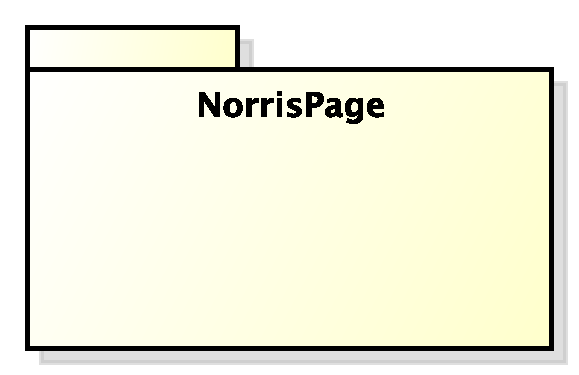
\includegraphics[scale=0.5]{DefinizioneDiProdotto/Pics/Classi/Norris--DataModel--NorrisPage}
				\caption{Norris::DataModel::NorrisPage}
			\end{figure}
		}
	

			\begin{itemize}
			\item \textbf{Nome:} NorrisPage
			\item \textbf{Tipo:} package
			
			\item \textbf{Descrizione:} NorrisPage è il package, le cui classi si occupano dell'aggiunta di grafici alle pagine e del settaggio delle impostazioni delle pagine.
			\end{itemize}

			
			\level{5}[PageImpl]{Norris::DataModel::NorrisPage::PageImpl}
			

		\IfFileExists{DefinizioneDiProdotto/Pics/Classi/Norris--DataModel--NorrisPage--PageImpl.pdf}{
			\begin{figure}[H]
				\centering
				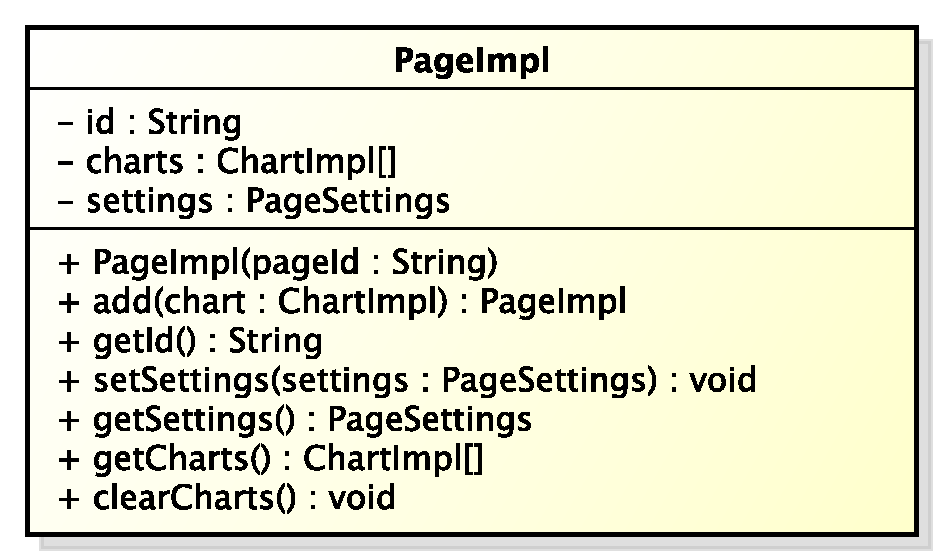
\includegraphics[scale=0.5]{DefinizioneDiProdotto/Pics/Classi/Norris--DataModel--NorrisPage--PageImpl}
				\caption{Norris::DataModel::NorrisPage::PageImpl}
			\end{figure}
		}
	
			
			\begin{itemize}
			\item \textbf{Nome:} PageImpl
			\item \textbf{Tipo:} classe
			
		\item \textbf{Astratta:}
		no
			\item \textbf{Visibilità:} public
			\item \textbf{Descrizione:} Questa classe rappresenta una pagina web. Essa contiene al suo interno dei grafici (ChartImpl) e le impostazioni della pagina web (PageSettingsObject).
			\item \textbf{Attributi:}
				\begin{itemize}
				\setlength{\itemsep}{5pt}
				
					\item[\ding{111}] {--id : String} \\ [1mm] Questo attributo consiste nell'id della pagina.
					\item[\ding{111}] {--charts : ChartImpl[]} \\ [1mm] Questo attributo consiste nell'insieme dei grafici contenuti nella pagina.
					\item[\ding{111}] {--settings : PageSettings} \\ [1mm] Questo attributo consiste nelle opzioni delle pagina rappresentata.
				\end{itemize}
		
			\item \textbf{Metodi:}
				\begin{itemize}
				\setlength{\itemsep}{5pt}
				
					\item[\ding{111}] {{+PageImpl(pageId : String)}} \\ [1mm] Questo metodo è il costruttore della classe. Il parametro rappresenta l'id che si vuole dare a atale pagina.
					\item[\ding{111}] {{+add(chart : ChartImpl) : PageImpl}} \\ [1mm] Questo metodo permette di aggiungere nuovi grafici alla pagina. Passando dunque come parametro un chart esso viene aggiunto alla pagina
					\item[\ding{111}] {{+getId() : String}} \\ [1mm] Questo metodo permette di ottenere l'id della pagina.
					\item[\ding{111}] {{+setSettings(settings : PageSettings) : void}} \\ [1mm] Questo metodo permette di impostare le opzioni della pagina.
					\item[\ding{111}] {{+getSettings() : PageSettings}} \\ [1mm] Questo metodo permette di ottenere le opzioni della pagina.
					\item[\ding{111}] {{+getCharts() : ChartImpl}} \\ [1mm] Questo metodo permette di ottenere la lista dei grafici contenuti nella pagina.
					\item[\ding{111}] {{+clearCharts() : void}} \\ [1mm] Questo metodo permette di togliere tutti i grafici contenuti nella pagina.
				\end{itemize}
		
			\end{itemize}

			
			\level{4}[InternalAPIManager]{Norris::InternalAPIManager}
			

		\IfFileExists{DefinizioneDiProdotto/Pics/Classi/Norris--InternalAPIManager.pdf}{
			\begin{figure}[H]
				\centering
				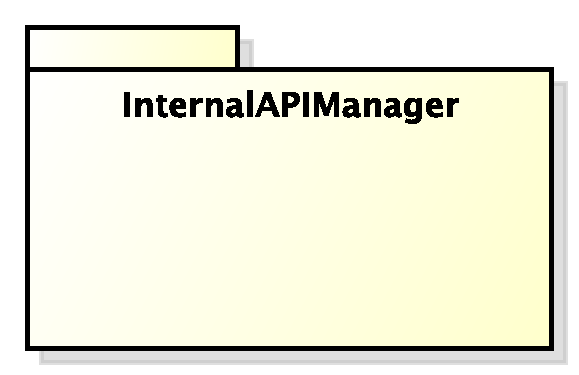
\includegraphics[scale=0.5]{DefinizioneDiProdotto/Pics/Classi/Norris--InternalAPIManager}
				\caption{Norris::InternalAPIManager}
			\end{figure}
		}
	

			\begin{itemize}
			\item \textbf{Nome:} InternalAPIManager
			\item \textbf{Tipo:} package
			
			\item \textbf{Descrizione:} InternalAPIManager è un package le cui classi si occupano di creare ed aggiornare grafici, creare pagine, aggiungere dei grafici ad esse o all'istanza di Norris e scegliere le varie impostazioni riguardanti grafici, pagine o istanze. Inoltre, forniscono le funzioni di autenticazione.
			\end{itemize}

			
			\level{5}[ChartBridge]{Norris::InternalAPIManager::ChartBridge}
			

		\IfFileExists{DefinizioneDiProdotto/Pics/Classi/Norris--InternalAPIManager--ChartBridge.pdf}{
			\begin{figure}[H]
				\centering
				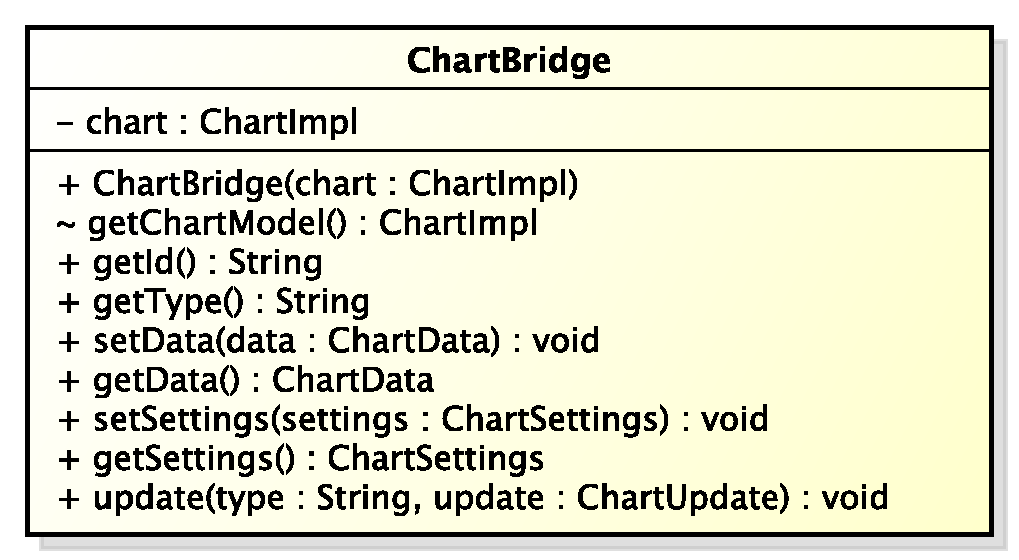
\includegraphics[scale=0.5]{DefinizioneDiProdotto/Pics/Classi/Norris--InternalAPIManager--ChartBridge}
				\caption{Norris::InternalAPIManager::ChartBridge}
			\end{figure}
		}
	
			
			\begin{itemize}
			\item \textbf{Nome:} ChartBridge
			\item \textbf{Tipo:} classe
			
		\item \textbf{Astratta:}
		no
			\item \textbf{Visibilità:} package
			\item \textbf{Descrizione:} ChartBridge implementa l'interfaccia Chart. Si occupa di inoltrare al modello dei dati le richieste di modifica delle impostazioni e le richieste di aggiornamento dei grafici.
			\item \textbf{Attributi:}
				\begin{itemize}
				\setlength{\itemsep}{5pt}
				
					\item[\ding{111}] {--chart : ChartImpl} \\ [1mm] Questo attributo è il riferimento all'istanza del chart rappresentato.
				\end{itemize}
		
			\item \textbf{Metodi:}
				\begin{itemize}
				\setlength{\itemsep}{5pt}
				
					\item[\ding{111}] {{+ChartBridge(chart : ChartImpl)}} \\ [1mm] Questo metodo è il costruttore della classe. esso salva il parametro nell'attributo chart.
					\item[\ding{111}] {{\(\sim\)getChartModel() : ChartImpl}} \\ [1mm] Questo metodo permette di ottenere il riferimento al chart rappresentato. Esso ritornerà il campo privato
					\item[\ding{111}] {{+getId() : String}} \\ [1mm] Questo metodo permette di ottenere l'id del chart rappresentato. Esso dovrà reperire tale informazione dal modello dei dati sfruttando l'attributo privato chart.
					\item[\ding{111}] {{+getType() : String}} \\ [1mm] Questo metodo permette di ottenere il tipo del chart rappresentato. Esso dovrà reperire tale informazione dal modello dei dati sfruttando l'attributo privato chart.
					\item[\ding{111}] {{+setData(data : ChartData) : void}} \\ [1mm] Questo metodo permette di impostare i dati del chart rappresentato.
					\item[\ding{111}] {{+getData() : ChartData}} \\ [1mm] Questo metodo permette di ottenere i dati del chart rappresentato. Esso dovrà reperire tale informazione dal modello dei dati sfruttando l'attributo privato chart.
					\item[\ding{111}] {{+setSettings(settings : ChartSettings) : void}} \\ [1mm] Questo metodo permette di impostare le opzioni del chart rappresentato.
					\item[\ding{111}] {{+getSettings() : ChartSettings}} \\ [1mm] Questo metodo permette di ottenere le opzioni del chart rappresentato. Esso dovrà reperire tale informazione dal modello dei dati sfruttando l'attributo privato chart.
					\item[\ding{111}] {{+update(type : String, update : ChartUpdate) : void}} \\ [1mm] Questo metodo permette di aggiornare il chart rappresentato secondo gli aggiornamenti previsti.
				\end{itemize}
		
			\end{itemize}

			
			\level{5}[NorrisBridge]{Norris::InternalAPIManager::NorrisBridge}
			

		\IfFileExists{DefinizioneDiProdotto/Pics/Classi/Norris--InternalAPIManager--NorrisBridge.pdf}{
			\begin{figure}[H]
				\centering
				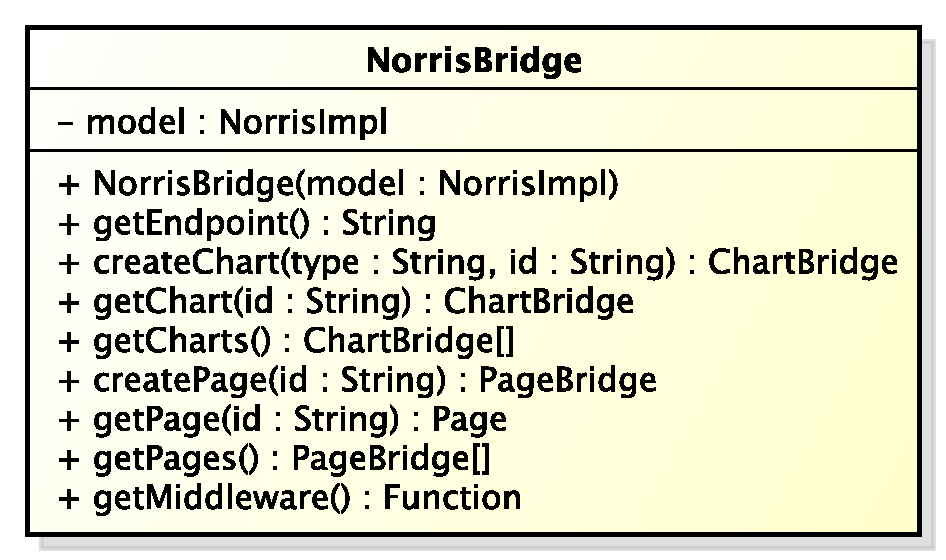
\includegraphics[scale=0.5]{DefinizioneDiProdotto/Pics/Classi/Norris--InternalAPIManager--NorrisBridge}
				\caption{Norris::InternalAPIManager::NorrisBridge}
			\end{figure}
		}
	
			
			\begin{itemize}
			\item \textbf{Nome:} NorrisBridge
			\item \textbf{Tipo:} classe
			
		\item \textbf{Astratta:}
		no
			\item \textbf{Visibilità:} public
			\item \textbf{Descrizione:} NorrisBridge implementa l'interfaccia Norris. Si occupa di inoltare al modello dei dati le richieste di modifica delle impostazioni e delle funzioni di autenticazione di un'istanza di Norris e le richieste di aggiunta di grafici e di pagine all'istanza stessa.
			\item \textbf{Attributi:}
				\begin{itemize}
				\setlength{\itemsep}{5pt}
				
					\item[\ding{111}] {--model : NorrisImpl} \\ [1mm] Questo attributo è il riferimento all'istanza di Norris rappresentata dalla classe.
				\end{itemize}
		
			\item \textbf{Metodi:}
				\begin{itemize}
				\setlength{\itemsep}{5pt}
				
					\item[\ding{111}] {{+NorrisBridge(model : NorrisImpl)}} \\ [1mm] Questo metodo è il costruttore della classe.
					\item[\ding{111}] {{+getEndpoint() : String}} \\ [1mm] Questo metodo permette di ottenere l'endpoint sul quale sono fornite le API. Esso reperirà tale informazione dal modello dei dati sfruttando l'attributo privato model.
					\item[\ding{111}] {{+createChart(type : String, id : String) : ChartBridge}} \\ [1mm] Questo metodo permette di creare un nuovo chart ed aggiungerlo all'istanza di Norris rappresentata.
					\item[\ding{111}] {{+getChart(id : String) : ChartBridge}} \\ [1mm] Questo metodo permette di ottenere un chart contenuto nell'istanza di Norris rappresentata tramite il suo id.
					\item[\ding{111}] {{+getCharts() : ChartBridge}} \\ [1mm] Questo metodo permette di ottenere l'insieme dei grafici presenti all'interno dell'istanza di Norris rappresentata.
					\item[\ding{111}] {{+createPage(id : String) : PageBridge}} \\ [1mm] Questo metodo permette di creare una nuova pagina ed aggiungerla all'istanza di Norris rappresentata.
					\item[\ding{111}] {{+getPage(id : String) : Page}} \\ [1mm] Questo metodo permette di ottenere una pagina contenuta nell'istanza di Norris rappresentata tramite il suo id.
					\item[\ding{111}] {{+getPages() : PageBridge[]}} \\ [1mm] Questo metodo permette di ottenere l'insieme delle pagine presenti all'interno dell'istanza di Norris rappresentata.
					\item[\ding{111}] {{+getMiddleware() : Function}} \\ [1mm] Questo metodo permette di ottenere un middleware per express, il quale consente di montare le pagine dell'instanza di Norris su un webserver.
				\end{itemize}
		
			\end{itemize}

			
			\level{5}[PageBridge]{Norris::InternalAPIManager::PageBridge}
			

		\IfFileExists{DefinizioneDiProdotto/Pics/Classi/Norris--InternalAPIManager--PageBridge.pdf}{
			\begin{figure}[H]
				\centering
				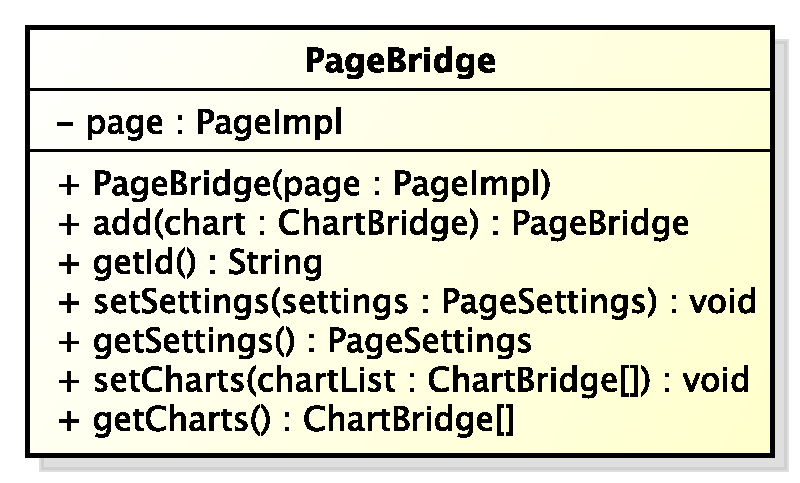
\includegraphics[scale=0.5]{DefinizioneDiProdotto/Pics/Classi/Norris--InternalAPIManager--PageBridge}
				\caption{Norris::InternalAPIManager::PageBridge}
			\end{figure}
		}
	
			
			\begin{itemize}
			\item \textbf{Nome:} PageBridge
			\item \textbf{Tipo:} classe
			
		\item \textbf{Astratta:}
		no
			\item \textbf{Visibilità:} package
			\item \textbf{Descrizione:} PageBridge implementa l'interfaccia Page. Si occupa di inoltare al modello dei dati le richieste di modifica delle impostazioni di una pagina e le richieste di aggiunta di grafici alla pagina stessa.
			\item \textbf{Attributi:}
				\begin{itemize}
				\setlength{\itemsep}{5pt}
				
					\item[\ding{111}] {--page : PageImpl} \\ [1mm] Questo attributo è un riferimento al tipo di pagina rappresentata.
				\end{itemize}
		
			\item \textbf{Metodi:}
				\begin{itemize}
				\setlength{\itemsep}{5pt}
				
					\item[\ding{111}] {{+PageBridge(page : PageImpl)}} \\ [1mm] Questo metodo è il costruttore della classe.	
					\item[\ding{111}] {{+add(chart : ChartBridge) : PageBridge}} \\ [1mm] Questo metodo permette di aggiungere nuovi chart alla pagina rappresentata.
					\item[\ding{111}] {{+getId() : String}} \\ [1mm] Questo metodo permette di ottenere l'id della pagina rappresentata.  Esso dovrà reperire tale informazione dal modello dei dati sfruttando l'attributo privato page.
					\item[\ding{111}] {{+setSettings(settings : PageSettings) : void}} \\ [1mm] Questo metodo permette di impostare le opzioni relative alla pagina rappresentata.
					\item[\ding{111}] {{+getSettings() : PageSettings}} \\ [1mm] Questo metodo permette di ottenere le opzioni della pagina rappresentata.  Esso dovrà reperire tale informazione dal modello dei dati sfruttando l'attributo privato page.
					\item[\ding{111}] {{+setCharts(chartList : ChartBridge[]) : void}} \\ [1mm] Questo metodo permette di impostare l'insieme dei chart contenuti nella pagina rappresentata.
					\item[\ding{111}] {{+getCharts() : ChartBridge[]}} \\ [1mm] Questo metodo permette di ottenere l'insieme dei chart contenuti nella pagina rappresentata. Esso dovrà reperire tale informazione dal modello dei dati sfruttando l'attributo privato page.
				\end{itemize}
		
			\end{itemize}

			
			\level{4}[ExternalAPIManager]{Norris::ExternalAPIManager}
			

		\IfFileExists{DefinizioneDiProdotto/Pics/Classi/Norris--ExternalAPIManager.pdf}{
			\begin{figure}[H]
				\centering
				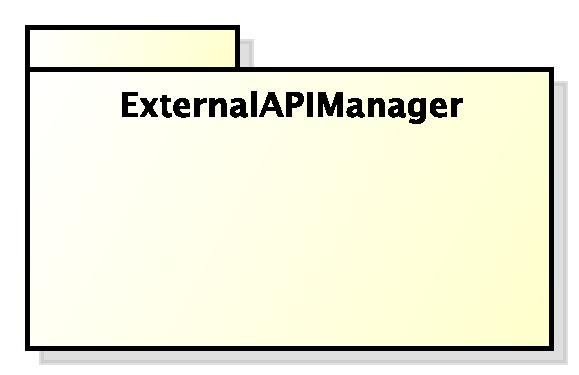
\includegraphics[scale=0.5]{DefinizioneDiProdotto/Pics/Classi/Norris--ExternalAPIManager}
				\caption{Norris::ExternalAPIManager}
			\end{figure}
		}
	

			\begin{itemize}
			\item \textbf{Nome:} ExternalAPIManager
			\item \textbf{Tipo:} package
			
			\item \textbf{Descrizione:} ExternalAPIManager è il package, le cui classi si occupano di implementare le funzionalità per: ottenere la lista dei grafici, ottenere un grafico con i relativi aggiornamenti ed effettuare login e logout. Inoltre, gestiscono la comunicazione con il websocket, tramite HTTP e canale Websocket.
			\end{itemize}

			
			\level{5}[AuthenticationEndpoint]{Norris::ExternalAPIManager::AuthenticationEndpoint}
			

		\IfFileExists{DefinizioneDiProdotto/Pics/Classi/Norris--ExternalAPIManager--AuthenticationEndpoint.pdf}{
			\begin{figure}[H]
				\centering
				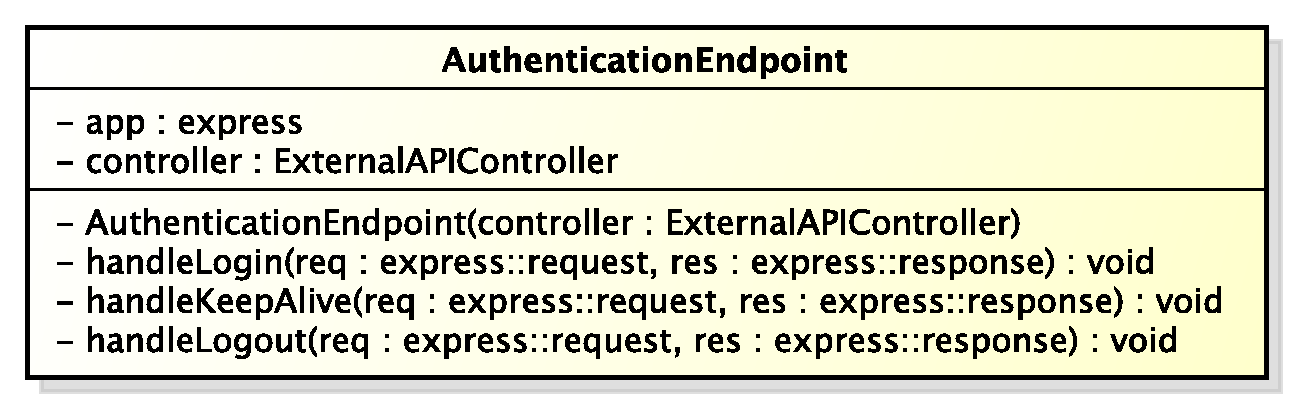
\includegraphics[scale=0.5]{DefinizioneDiProdotto/Pics/Classi/Norris--ExternalAPIManager--AuthenticationEndpoint}
				\caption{Norris::ExternalAPIManager::AuthenticationEndpoint}
			\end{figure}
		}
	
			
			\begin{itemize}
			\item \textbf{Nome:} AuthenticationEndpoint
			\item \textbf{Tipo:} classe
			
		\item \textbf{Astratta:}
		no
			\item \textbf{Visibilità:} package
			\item \textbf{Descrizione:} Questa classe si occupa di gestire l'autenticazione. In particolare si occupa di gestire le richieste di login e di logout, eseguendo le funzioni definite dallo sviluppatore e contenute in NorrisImpl.
			\item \textbf{Attributi:}
				\begin{itemize}
				\setlength{\itemsep}{5pt}
				
					\item[\ding{111}] {--controller : ExternalAPIController} \\ [1mm] Questo attributo è un riferimento all'oggetto che permette di ricavare informazioni sull'istanza di Norris.
				\end{itemize}
		
			\item \textbf{Metodi:}
				\begin{itemize}
				\setlength{\itemsep}{5pt}
				
					\item[\ding{111}] {{--AuthenticationEndpoint(controller : ExternalAPIController)}} \\ [1mm] Questo metodo è il costruttore della classe.
					\item[\ding{111}] {{--handleLogin(req : express::request, res : express::response) : void}} \\ [1mm] Questo metodo gestisce una richiesta di autenticazione. La richiesta HTTP ricevuta viene demandata all'ExternalAPIController che effettuerà il login.
					\item[\ding{111}] {{--handleKeepAlive(req : express::request, res : express::response) : void}} \\ [1mm] Questo metodo gestisce una richiesta per il rinnovo della sessione. La richiesta HTTP ricevuta viene demandata all'ExternalAPIController che effettuerà il mantenimento della sessione.
					\item[\ding{111}] {{--handleLogout(req : express::request, res : express::response) : void}} \\ [1mm] Questo metodo gestisce una richiesta per la terminazione della sessione. La richiesta HTTP ricevuta viene demandata all'ExternalAPIController che effettuerà il logout.
				\end{itemize}
		
			\end{itemize}

			
			\level{5}[AuthenticationEndpointFactory]{Norris::ExternalAPIManager::AuthenticationEndpoint::AuthenticationEndpointFactory}
			

		\IfFileExists{DefinizioneDiProdotto/Pics/Classi/Norris--ExternalAPIManager--AuthenticationEndpoint--AuthenticationEndpointFactory.pdf}{
			\begin{figure}[H]
				\centering
				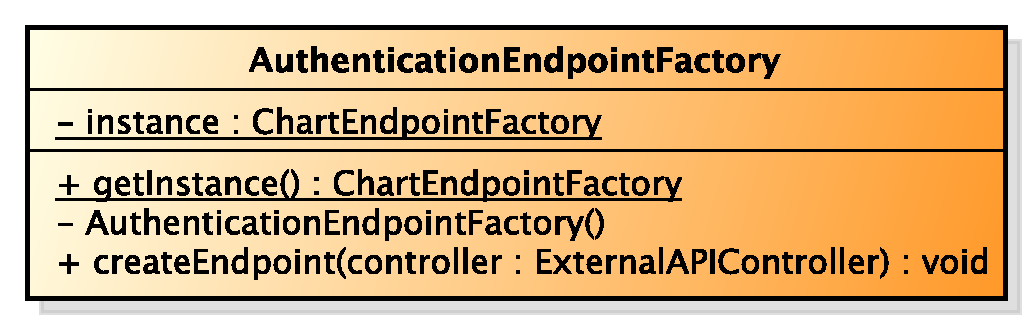
\includegraphics[scale=0.5]{DefinizioneDiProdotto/Pics/Classi/Norris--ExternalAPIManager--AuthenticationEndpoint--AuthenticationEndpointFactory}
				\caption{Norris::ExternalAPIManager::AuthenticationEndpoint::AuthenticationEndpointFactory}
			\end{figure}
		}
	
			
			\begin{itemize}
			\item \textbf{Nome:} AuthenticationEndpointFactory
			\item \textbf{Tipo:} classe
			
		\item \textbf{Astratta:}
		no
			\item \textbf{Visibilità:} private
			\item \textbf{Descrizione:} Questa classe si occupa della creazione di un endpoint di tipo AuthenticationEndpoint. Tale classe dispone di un blocco di inizializzazione statica che registra la sua istanza nell'array endpoints della classe ExternalAPIConstructor non appena tale classe viene caricata.
			\item \textbf{Attributi:}
				\begin{itemize}
				\setlength{\itemsep}{5pt}
				
					\item[\ding{111}] \underline{--instance : ChartEndpointFactory} \\ [1mm] Questo attributo è il riferimento all'unica istanza della classe.
				\end{itemize}
		
			\item \textbf{Metodi:}
				\begin{itemize}
				\setlength{\itemsep}{5pt}
				
					\item[\ding{111}] {\underline{+getInstance() : ChartEndpointFactory}} \\ [1mm] Questo metodo permette di ottenere l'unica istanza esistente della classe.
					\item[\ding{111}] {{--AuthenticationEndpointFactory()}} \\ [1mm] Questo metodo è il costruttore della classe. Esso è privato perchè non si vuole permettere a nessuno di poter creare un’istanza se non utilizzando il metodo getInstance().

					\item[\ding{111}] {{+createEndpoint(controller : ExternalAPIController) : void}} \\ [1mm] Questo metodo crea un'istanza della classe AuthenticationEndpoint.
				\end{itemize}
		
			\end{itemize}

			
			\level{5}[ChartEndpoint]{Norris::ExternalAPIManager::ChartEndpoint}
			

		\IfFileExists{DefinizioneDiProdotto/Pics/Classi/Norris--ExternalAPIManager--ChartEndpoint.pdf}{
			\begin{figure}[H]
				\centering
				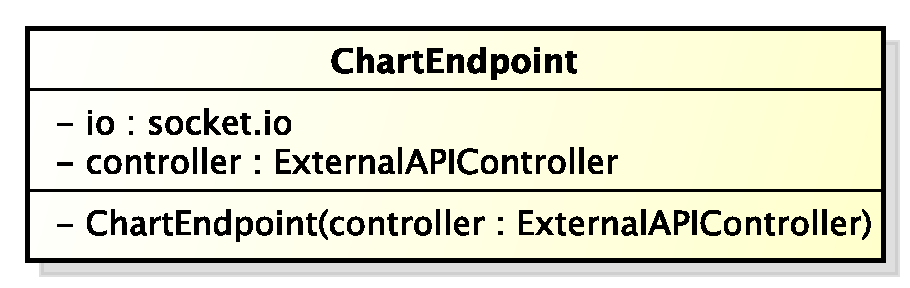
\includegraphics[scale=0.5]{DefinizioneDiProdotto/Pics/Classi/Norris--ExternalAPIManager--ChartEndpoint}
				\caption{Norris::ExternalAPIManager::ChartEndpoint}
			\end{figure}
		}
	
			
			\begin{itemize}
			\item \textbf{Nome:} ChartEndpoint
			\item \textbf{Tipo:} classe
			
		\item \textbf{Astratta:}
		no
			\item \textbf{Visibilità:} package
			\item \textbf{Descrizione:} Questa classe si occupa di gestire le richieste di  grafici da parte dei client, nonchè l'invio degli aggiornamenti dei grafici stessi. In particolare, ad ogni richiesta di un grafico controlla se il client è autenticato all'istanza di Norris. Essa contiene un oggetto del modulo socket.io di Node.js per gestire l'invio dei grafici e degli aggiornamenti tramite canale websocket.
			\item \textbf{Attributi:}
				\begin{itemize}
				\setlength{\itemsep}{5pt}
				
					\item[\ding{111}] {--io : socket.io} \\ [1mm] Questo attributo è un riferimento ad un'istanza di socket.io, utilizzata per fornire le funzionalità.
					\item[\ding{111}] {--controller : ExternalAPIController} \\ [1mm] Questo attributo è un riferimento all'oggetto che permette di ricavare informazioni sull'istanza di Norris.
				\end{itemize}
		
			\item \textbf{Metodi:}
				\begin{itemize}
				\setlength{\itemsep}{5pt}
				
					\item[\ding{111}] {{--ChartEndpoint(controller : ExternalAPIController)}} \\ [1mm] Questo metodo è il costruttore della classe.
				\end{itemize}
		
			\end{itemize}

			
			\level{5}[ChartEndpointFactory]{Norris::ExternalAPIManager::ChartEndpoint::ChartEndpointFactory}
			

		\IfFileExists{DefinizioneDiProdotto/Pics/Classi/Norris--ExternalAPIManager--ChartEndpoint--ChartEndpointFactory.pdf}{
			\begin{figure}[H]
				\centering
				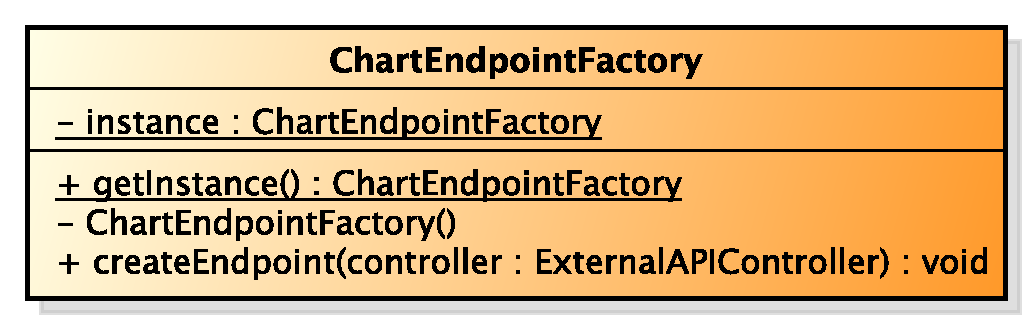
\includegraphics[scale=0.5]{DefinizioneDiProdotto/Pics/Classi/Norris--ExternalAPIManager--ChartEndpoint--ChartEndpointFactory}
				\caption{Norris::ExternalAPIManager::ChartEndpoint::ChartEndpointFactory}
			\end{figure}
		}
	
			
			\begin{itemize}
			\item \textbf{Nome:} ChartEndpointFactory
			\item \textbf{Tipo:} classe
			
		\item \textbf{Astratta:}
		no
			\item \textbf{Visibilità:} private
			\item \textbf{Descrizione:} Questa classe si occupa della creazione di un endpoint di tipo ChartEndpoint.  Tale classe dispone di un blocco di inizializzazione statica che registra la sua istanza nell'array endpoints della classe ExternalAPIConstructor non appena tale classe viene caricata.
			\item \textbf{Attributi:}
				\begin{itemize}
				\setlength{\itemsep}{5pt}
				
					\item[\ding{111}] \underline{--instance : ChartEndpointFactory} \\ [1mm] Questo attributo è il riferimento all'unica istanza della classe.
				\end{itemize}
		
			\item \textbf{Metodi:}
				\begin{itemize}
				\setlength{\itemsep}{5pt}
				
					\item[\ding{111}] {\underline{+getInstance() : ChartEndpointFactory}} \\ [1mm] Questo metodo permette di ottenere l'unica istanza esistente della classe.
					\item[\ding{111}] {{--ChartEndpointFactory()}} \\ [1mm] Questo metodo è il costruttore della classe. Esso è privato perchè non si vuole permettere a nessuno di poter creare un’istanza se non utilizzando il metodo getInstance().

					\item[\ding{111}] {{+createEndpoint(controller : ExternalAPIController) : void}} \\ [1mm] Questo metodo crea un'istanza della classe ChartEndpoint.
				\end{itemize}
		
			\end{itemize}

			
			\level{5}[ChartRef]{Norris::ExternalAPIManager::ChartRef}
			

		\IfFileExists{DefinizioneDiProdotto/Pics/Classi/Norris--ExternalAPIManager--ChartRef.pdf}{
			\begin{figure}[H]
				\centering
				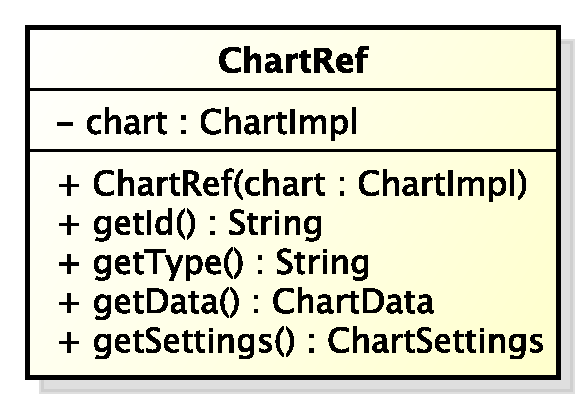
\includegraphics[scale=0.5]{DefinizioneDiProdotto/Pics/Classi/Norris--ExternalAPIManager--ChartRef}
				\caption{Norris::ExternalAPIManager::ChartRef}
			\end{figure}
		}
	
			
			\begin{itemize}
			\item \textbf{Nome:} ChartRef
			\item \textbf{Tipo:} classe
			
		\item \textbf{Estende:}
		EventEmitter
		\item \textbf{Astratta:}
		no
			\item \textbf{Visibilità:} package
			\item \textbf{Descrizione:} Questa classe contiene un riferimento ad un oggetto di tipo ChartModel. È presente un'istanza di ChartRef per ognuno dei grafici dell'istanza di Norris che sono stati richiesti tramite API esterne.
			\item \textbf{Attributi:}
				\begin{itemize}
				\setlength{\itemsep}{5pt}
				
					\item[\ding{111}] {--chart : ChartImpl} \\ [1mm] Questo attributo è un riferimento al chart di Norris rappresentato.
				\end{itemize}
		
			\item \textbf{Metodi:}
				\begin{itemize}
				\setlength{\itemsep}{5pt}
				
					\item[\ding{111}] {{+ChartRef(chart : ChartImpl)}}
					\item[\ding{111}] {{+getId() : String}} \\ [1mm] Questo metodo è il costruttore della classe. Esso dovrà reperire tale informazione dal modello dei dati sfruttando l'attributo privato chart.
					\item[\ding{111}] {{+getType() : String}} \\ [1mm] Questo metodo permette di ottenere il tipo del grafico rappresento. Esso dovrà reperire tale informazione dal modello dei dati sfruttando l'attributo privato chart.
					\item[\ding{111}] {{+getData() : ChartData}} \\ [1mm] Questo metodo permette di ottenere i dati del grafico rappresentato. Esso dovrà reperire tale informazione dal modello dei dati sfruttando l'attributo privato chart.
					\item[\ding{111}] {{+getSettings() : ChartSettings}} \\ [1mm] Questo metodo permette di ottenere le opzioni del grafico rappresentato. Esso dovrà reperire tale informazione dal modello dei dati sfruttando l'attributo privato chart.
				\end{itemize}
		
			\end{itemize}

			
			\level{5}[ExternalAPIConstructor]{Norris::ExternalAPIManager::ExternalAPIConstructor}
			

		\IfFileExists{DefinizioneDiProdotto/Pics/Classi/Norris--ExternalAPIManager--ExternalAPIConstructor.pdf}{
			\begin{figure}[H]
				\centering
				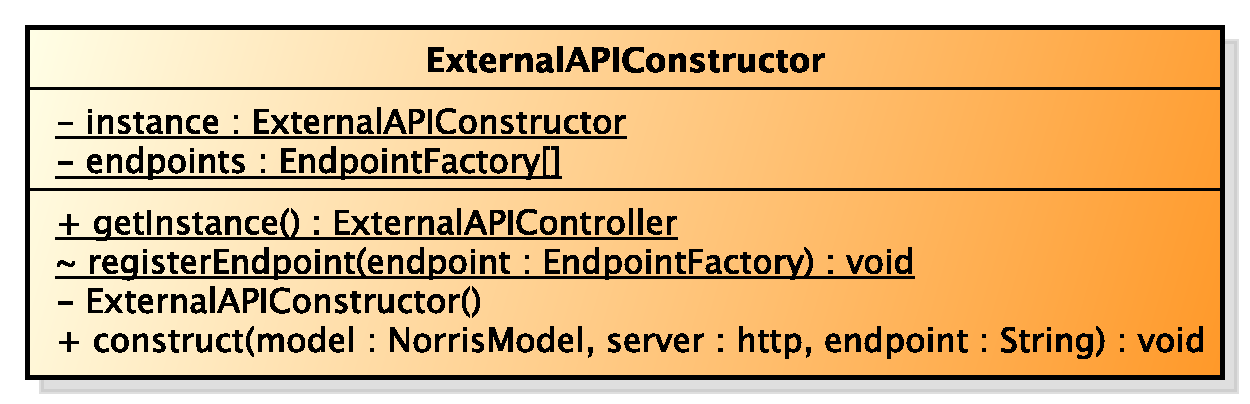
\includegraphics[scale=0.5]{DefinizioneDiProdotto/Pics/Classi/Norris--ExternalAPIManager--ExternalAPIConstructor}
				\caption{Norris::ExternalAPIManager::ExternalAPIConstructor}
			\end{figure}
		}
	
			
			\begin{itemize}
			\item \textbf{Nome:} ExternalAPIConstructor
			\item \textbf{Tipo:} classe
			
		\item \textbf{Astratta:}
		no
			\item \textbf{Visibilità:} public
			\item \textbf{Descrizione:} Questa classe ha la funzione di costruire la componente ExternalAPIManager. Dopo aver creato un'istanza di ExternalAPIController, viene creato un endpoint per ogni dipendenza salvata nell'attributo endpoints.
			\item \textbf{Attributi:}
				\begin{itemize}
				\setlength{\itemsep}{5pt}
				
					\item[\ding{111}] \underline{--instance : ExternalAPIConstructor} \\ [1mm] Questo attributo è il riferimento all'unica istanza della classe.
					\item[\ding{111}] \underline{--endpoints : EndpointFactory[]} \\ [1mm] Questo attributo contiene le dipendenze necessarie per costruire gli endpoint.
				\end{itemize}
		
			\item \textbf{Metodi:}
				\begin{itemize}
				\setlength{\itemsep}{5pt}
				
					\item[\ding{111}] {\underline{+getInstance() : ExternalAPIConstructor}} \\ [1mm] Questo metodo permette di ottenere l'unica istanza esistente della classe.
					\item[\ding{111}] {\underline{\(\sim\)registerEndpoint(endpoint : EndpointFactory) : void}} \\ [1mm] Questo metodo permette di registrare le dipendenze per la creazione di nuovi endpoint. Tale metodo permette alle factory di registrarsi nel vettore delle factory (endpoints) permettendone così l'utilizzo.
					\item[\ding{111}] {{--ExternalAPIConstructor()}} \\ [1mm] Questo metodo è il costruttore della classe.  Esso è privato perchè non si vuole permettere a nessuno di poter creare un’istanza se non utilizzando il metodo getInstance().

					\item[\ding{111}] {{+construct(model : NorrisImpl, server : http, app : express) : void}} \\ [1mm] Questo metodo permette di costruire la componente ExternalAPIManager in funzione dei parametri passati.
				\end{itemize}
		
			\end{itemize}

			
			\level{5}[ExternalAPIController]{Norris::ExternalAPIManager::ExternalAPIController}
			

		\IfFileExists{DefinizioneDiProdotto/Pics/Classi/Norris--ExternalAPIManager--ExternalAPIController.pdf}{
			\begin{figure}[H]
				\centering
				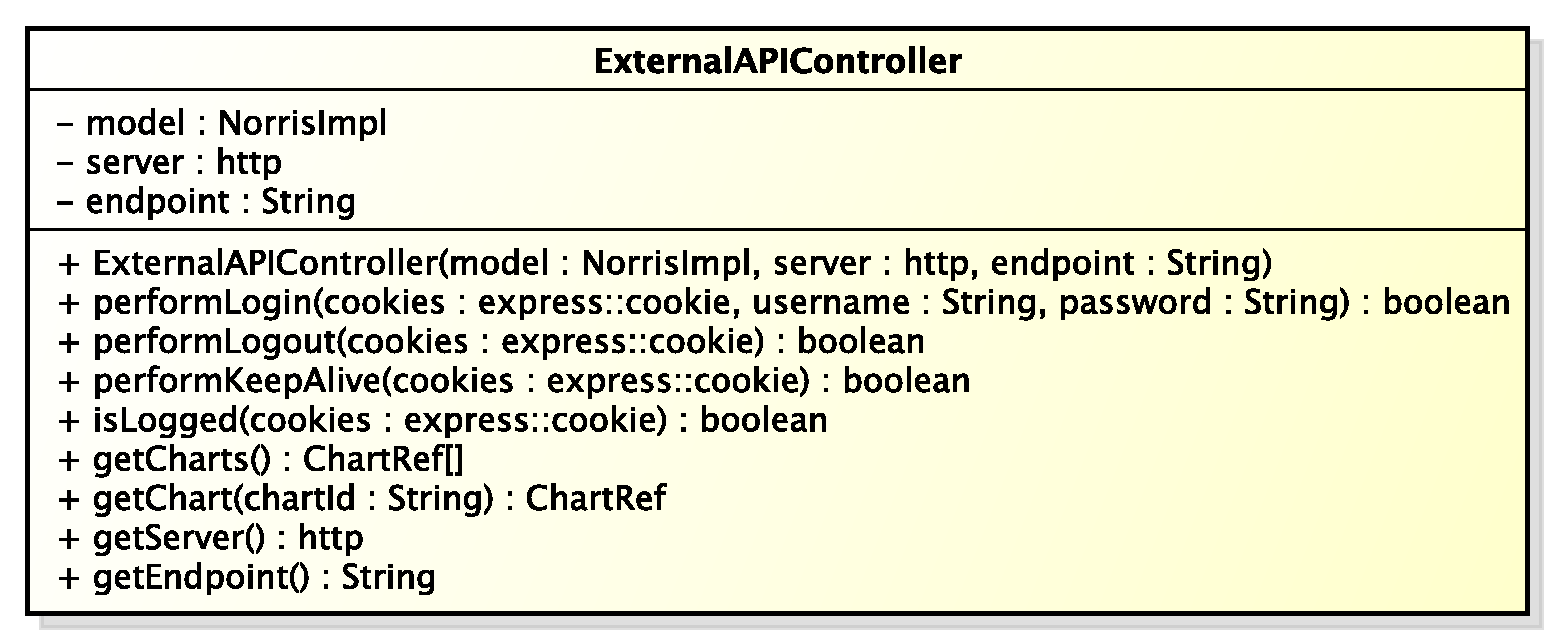
\includegraphics[scale=0.5]{DefinizioneDiProdotto/Pics/Classi/Norris--ExternalAPIManager--ExternalAPIController}
				\caption{Norris::ExternalAPIManager::ExternalAPIController}
			\end{figure}
		}
	
			
			\begin{itemize}
			\item \textbf{Nome:} ExternalAPIController
			\item \textbf{Tipo:} classe
			
		\item \textbf{Estende:}
		EventEmitter
		\item \textbf{Astratta:}
		no
			\item \textbf{Visibilità:} package
			\item \textbf{Descrizione:} Al suo interno ci sono un riferimento al NorrisModel ed un riferimento ad un oggetto del modulo http di Node.js. Contiene inoltre l'interfaccia EndPointFactory.
			\item \textbf{Attributi:}
				\begin{itemize}
				\setlength{\itemsep}{5pt}
				
					\item[\ding{111}] {--model : NorrisImpl} \\ [1mm] Questo attributo è un riferimento al modello di Norris sul quale si basa la componente ExternalAPIManager.
					\item[\ding{111}] {--server : http} \\ [1mm] Questo attributo è l'istanza del webserver che la componente utilizza per offrire le sue funzionalità.
					\item[\ding{111}] {--app : express}
				\end{itemize}
		
			\item \textbf{Metodi:}
				\begin{itemize}
				\setlength{\itemsep}{5pt}
				
					\item[\ding{111}] {{+ExternalAPIController(model : NorrisImpl, server : http, app : express)}} \\ [1mm] Questo metodo è il costruttore della classe.
					\item[\ding{111}] {{+performLogin(cookies : express::cookie, username : String, password : String) : boolean}} \\ [1mm] Questo metodo avvia una nuova sessione per l'utente e permette di impostare il token tramite il parametro cookies. 
					\item[\ding{111}] {{+performLogout(cookies : express::cookie) : boolean}} \\ [1mm] Questo metodo permette di terminare la sessione di un utente mediante i cookie passati come parametro.
					\item[\ding{111}] {{+performKeepAlive(cookies : express::cookie) : boolean}} \\ [1mm] Questo metodo permette di rinnovare la sessione di un utente mediante i cookie passati come parametro.
					\item[\ding{111}] {{+isLogged(cookies : express::cookie) : boolean}} \\ [1mm] Questo metodo permette di verificare se l'utente è autenticato tramite i cookie passati come parametro.
					\item[\ding{111}] {{+getCharts() : ChartRef[]}} \\ [1mm] Questo metodo permette di ottenere una lista di tutti i grafici presenti nell'istanza di Norris rappresentata.
					\item[\ding{111}] {{+getChart(chartId : String) : ChartRef}} \\ [1mm] Questo metodo permette di ottenere un chart contenuto nell'istanza di Norris rappresentata tramite il suo id.
					\item[\ding{111}] {{+getServer() : http}} \\ [1mm] Questo metodo permette di ottenere il server.
					\item[\ding{111}] {{+getEndpoint() : String}} \\ [1mm] Questo metodo permette di ottenere l'endpoint sul quale sono fornite le API.
					\item[\ding{111}] {{+getApp() : express}}
				\end{itemize}
		
			\end{itemize}

			
			\level{5}[ListEndpoint]{Norris::ExternalAPIManager::ListEndpoint}
			

		\IfFileExists{DefinizioneDiProdotto/Pics/Classi/Norris--ExternalAPIManager--ListEndpoint.pdf}{
			\begin{figure}[H]
				\centering
				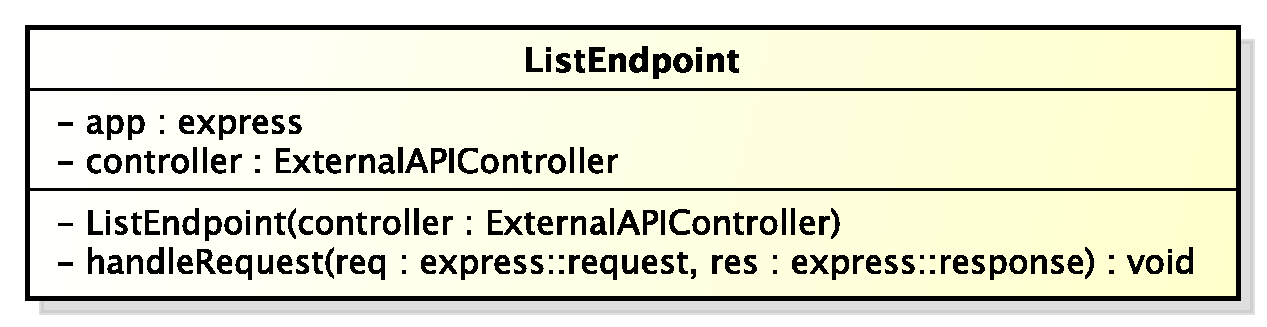
\includegraphics[scale=0.5]{DefinizioneDiProdotto/Pics/Classi/Norris--ExternalAPIManager--ListEndpoint}
				\caption{Norris::ExternalAPIManager::ListEndpoint}
			\end{figure}
		}
	
			
			\begin{itemize}
			\item \textbf{Nome:} ListEndpoint
			\item \textbf{Tipo:} classe
			
		\item \textbf{Astratta:}
		no
			\item \textbf{Visibilità:} package
			\item \textbf{Descrizione:} Questa classe si occupa di gestire le richieste della lista dei  grafici da parte dei client. In particolare, ad ogni richiesta della lista controlla se il client è autenticato all'istanza di Norris. Essa contiene un oggetto del modulo express di Node.js per gestire l'invio della lista di grafici tramite richiesta HTTP.
			\item \textbf{Attributi:}
				\begin{itemize}
				\setlength{\itemsep}{5pt}
				
					\item[\ding{111}] {--controller : ExternalAPIController} \\ [1mm] Questo attributo è un riferimento all'oggetto che permette di ricavare informazioni sull'istanza di Norris.
				\end{itemize}
		
			\item \textbf{Metodi:}
				\begin{itemize}
				\setlength{\itemsep}{5pt}
				
					\item[\ding{111}] {{--ListEndpoint(controller : ExternalAPIController)}} \\ [1mm] Questo metodo è il costruttore della classe.
					\item[\ding{111}] {{--handleRequest(req : express::request, res : express::response) : void}} \\ [1mm] Questo metodo gestisce una richiesta per l'ottenimento della lista dei grafici.
				\end{itemize}
		
			\end{itemize}

			
			\level{5}[ListEndpointFactory]{Norris::ExternalAPIManager::ListEndpoint::ListEndpointFactory}
			

		\IfFileExists{DefinizioneDiProdotto/Pics/Classi/Norris--ExternalAPIManager--ListEndpoint--ListEndpointFactory.pdf}{
			\begin{figure}[H]
				\centering
				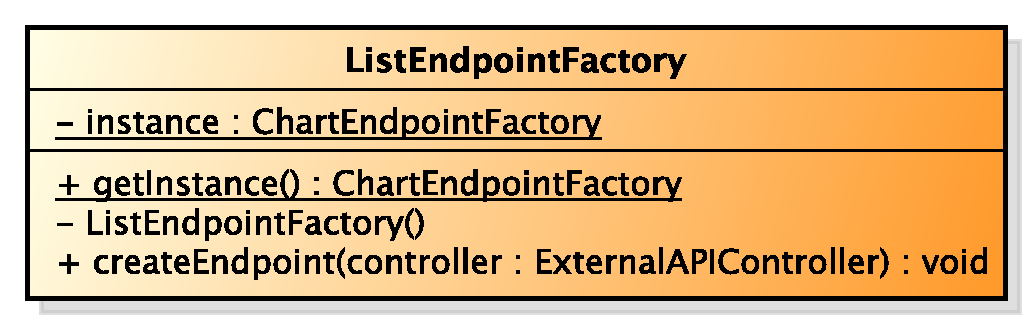
\includegraphics[scale=0.5]{DefinizioneDiProdotto/Pics/Classi/Norris--ExternalAPIManager--ListEndpoint--ListEndpointFactory}
				\caption{Norris::ExternalAPIManager::ListEndpoint::ListEndpointFactory}
			\end{figure}
		}
	
			
			\begin{itemize}
			\item \textbf{Nome:} ListEndpointFactory
			\item \textbf{Tipo:} classe
			
		\item \textbf{Astratta:}
		no
			\item \textbf{Visibilità:} private
			\item \textbf{Descrizione:} Questa classe si occupa della creazione di un endpoint di tipo ListEndpoint. Tale classe dispone di un blocco di inizializzazione statica che registra la sua istanza nell'array endpoints della classe ExternalAPIConstructor non appena tale classe viene caricata.
			\item \textbf{Attributi:}
				\begin{itemize}
				\setlength{\itemsep}{5pt}
				
					\item[\ding{111}] \underline{--instance : ChartEndpointFactory} \\ [1mm] Questo attributo è il riferimento all'unica istanza della classe.
				\end{itemize}
		
			\item \textbf{Metodi:}
				\begin{itemize}
				\setlength{\itemsep}{5pt}
				
					\item[\ding{111}] {\underline{+getInstance() : ChartEndpointFactory}} \\ [1mm] Questo metodo permette di ottenere l'unica istanza esistente della classe.
					\item[\ding{111}] {{--ListEndpointFactory()}} \\ [1mm] Questo metodo è il costruttore della classe. Esso è privato perchè non si vuole permettere a nessuno di poter creare un’istanza se non utilizzando il metodo getInstance().

					\item[\ding{111}] {{+createEndpoint(controller : ExternalAPIController) : void}} \\ [1mm] Questo metodo crea un'istanza della classe ListtEndpoint.
				\end{itemize}
		
			\end{itemize}

			
        
			\level{4}[NorrisSettingsImpl]{NorrisAggiuntive::NorrisSettingsImpl}
			

		\IfFileExists{DefinizioneDiProdotto/Pics/ClassiAggiuntive/NorrisSettingsImpl.pdf}{
			\begin{figure}[H]
				\centering
				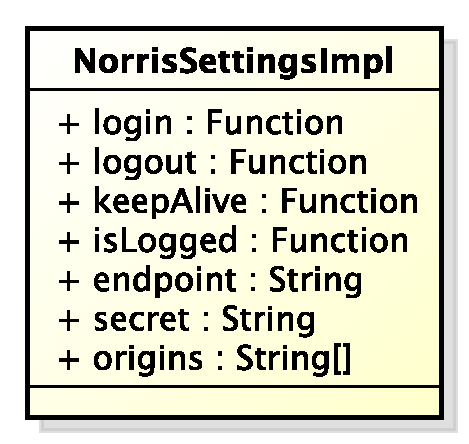
\includegraphics[scale=0.5]{DefinizioneDiProdotto/Pics/ClassiAggiuntive/NorrisSettingsImpl}
				\caption{NorrisSettingsImpl}
			\end{figure}
		}
	
			
			\begin{itemize}
			\item \textbf{Nome:} NorrisSettingsImpl
			\item \textbf{Tipo:} classe
			
		\item \textbf{Astratta:}
		no
			\item \textbf{Visibilità:} public
			\item \textbf{Descrizione:} La classe NorrisSettingsImpl definisce le impostazioni relative ad un'istanza di Norris. Lo sviluppatore può definire le funzioni che verranno eseguite per l'autenticazione.
			\item \textbf{Attributi:}
				\begin{itemize}
				\setlength{\itemsep}{5pt}
				
					\item[\ding{111}] {+login : Function} \\ [1mm] L'attributo login rappresenta la funzione che verrà eseguita per avviare la sessione di un utente.
					\item[\ding{111}] {+logout : Function} \\ [1mm] L'attributo login rappresenta la funzione che verrà eseguita per terminare la sessione di un utente.
					\item[\ding{111}] {+keepAlive : Function} \\ [1mm] L'attributo login rappresenta la funzione che verrà eseguita per rinnovare la sessione di un utente.
					\item[\ding{111}] {+isLogged : Function} \\ [1mm] L'attributo login rappresenta la funzione che verrà eseguita per verificare lo stato dela sessione di un utente.
					\item[\ding{111}] {+endpoint : String} \\ [1mm] L'attributo endpoint definisce il path al quale sono disponibili le API esterne.
					\item[\ding{111}] {+secret : String} \\ [1mm] L'attributo secret definisce la chiave di cifrature per i cookie firmati.
					\item[\ding{111}] {+origins : String[]} \\ [1mm] L'attributo origin definisce gli host attendibili, verso i quali saranno disponibili le API esterne.
				\end{itemize}
		
			\end{itemize}
	
			\level{4}[PageSettingsImpl]{NorrisAggiuntive::PageSettingsImpl}
			

		\IfFileExists{DefinizioneDiProdotto/Pics/ClassiAggiuntive/PageSettingsImpl.pdf}{
			\begin{figure}[H]
				\centering
				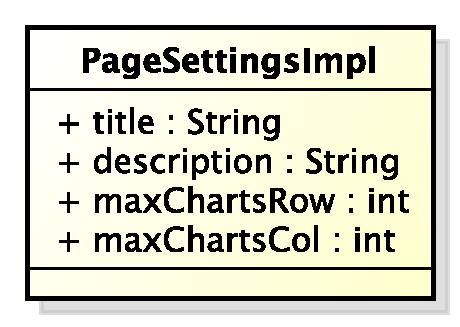
\includegraphics[scale=0.5]{DefinizioneDiProdotto/Pics/ClassiAggiuntive/PageSettingsImpl}
				\caption{PageSettingsImpl}
			\end{figure}
		}
	
			
			\begin{itemize}
			\item \textbf{Nome:} PageSettingsImpl
			\item \textbf{Tipo:} classe
			
		\item \textbf{Astratta:}
		no
			\item \textbf{Visibilità:} public
			\item \textbf{Descrizione:} La classe PageSettingsImpl definisce le impostazioni di una pagina di Norris.
			\item \textbf{Attributi:}
				\begin{itemize}
				\setlength{\itemsep}{5pt}
				
					\item[\ding{111}] {+title : String} \\ [1mm] L'attributo title rappresenta il titolo di una pagina di Norris.
					\item[\ding{111}] {+maxChartsRow : int} \\ [1mm] L'attributo title rappresenta il numero massimo di righe visualizzabili all'interno della pagina.
					\item[\ding{111}] {+maxChartsCol : int} \\ [1mm] L'attributo title rappresenta il numero massimo di colonne visualizzabili all'interno della pagina.
				\end{itemize}
		
			\end{itemize}
	

    \level{2}{Diagrammi di sequenza}
    	In tale sezione vengono presentati i diagrammi di sequenza, che hanno lo scopo di descrivere scenari (determinate sequenze di azioni in cui tutte le scelte sono già state effettuate). Essi vengono usati per descrivere le relazioni che intercorrono, in termini di messaggi, tra attori, oggetti ed entità del sistema \insglo{Norris}.
        \level{3}{Creazione di un chart}
        	Tale diagramma descrive come viene creato un chart di un certo tipo prefissato.
            \begin{figure}[H]
                \centering
                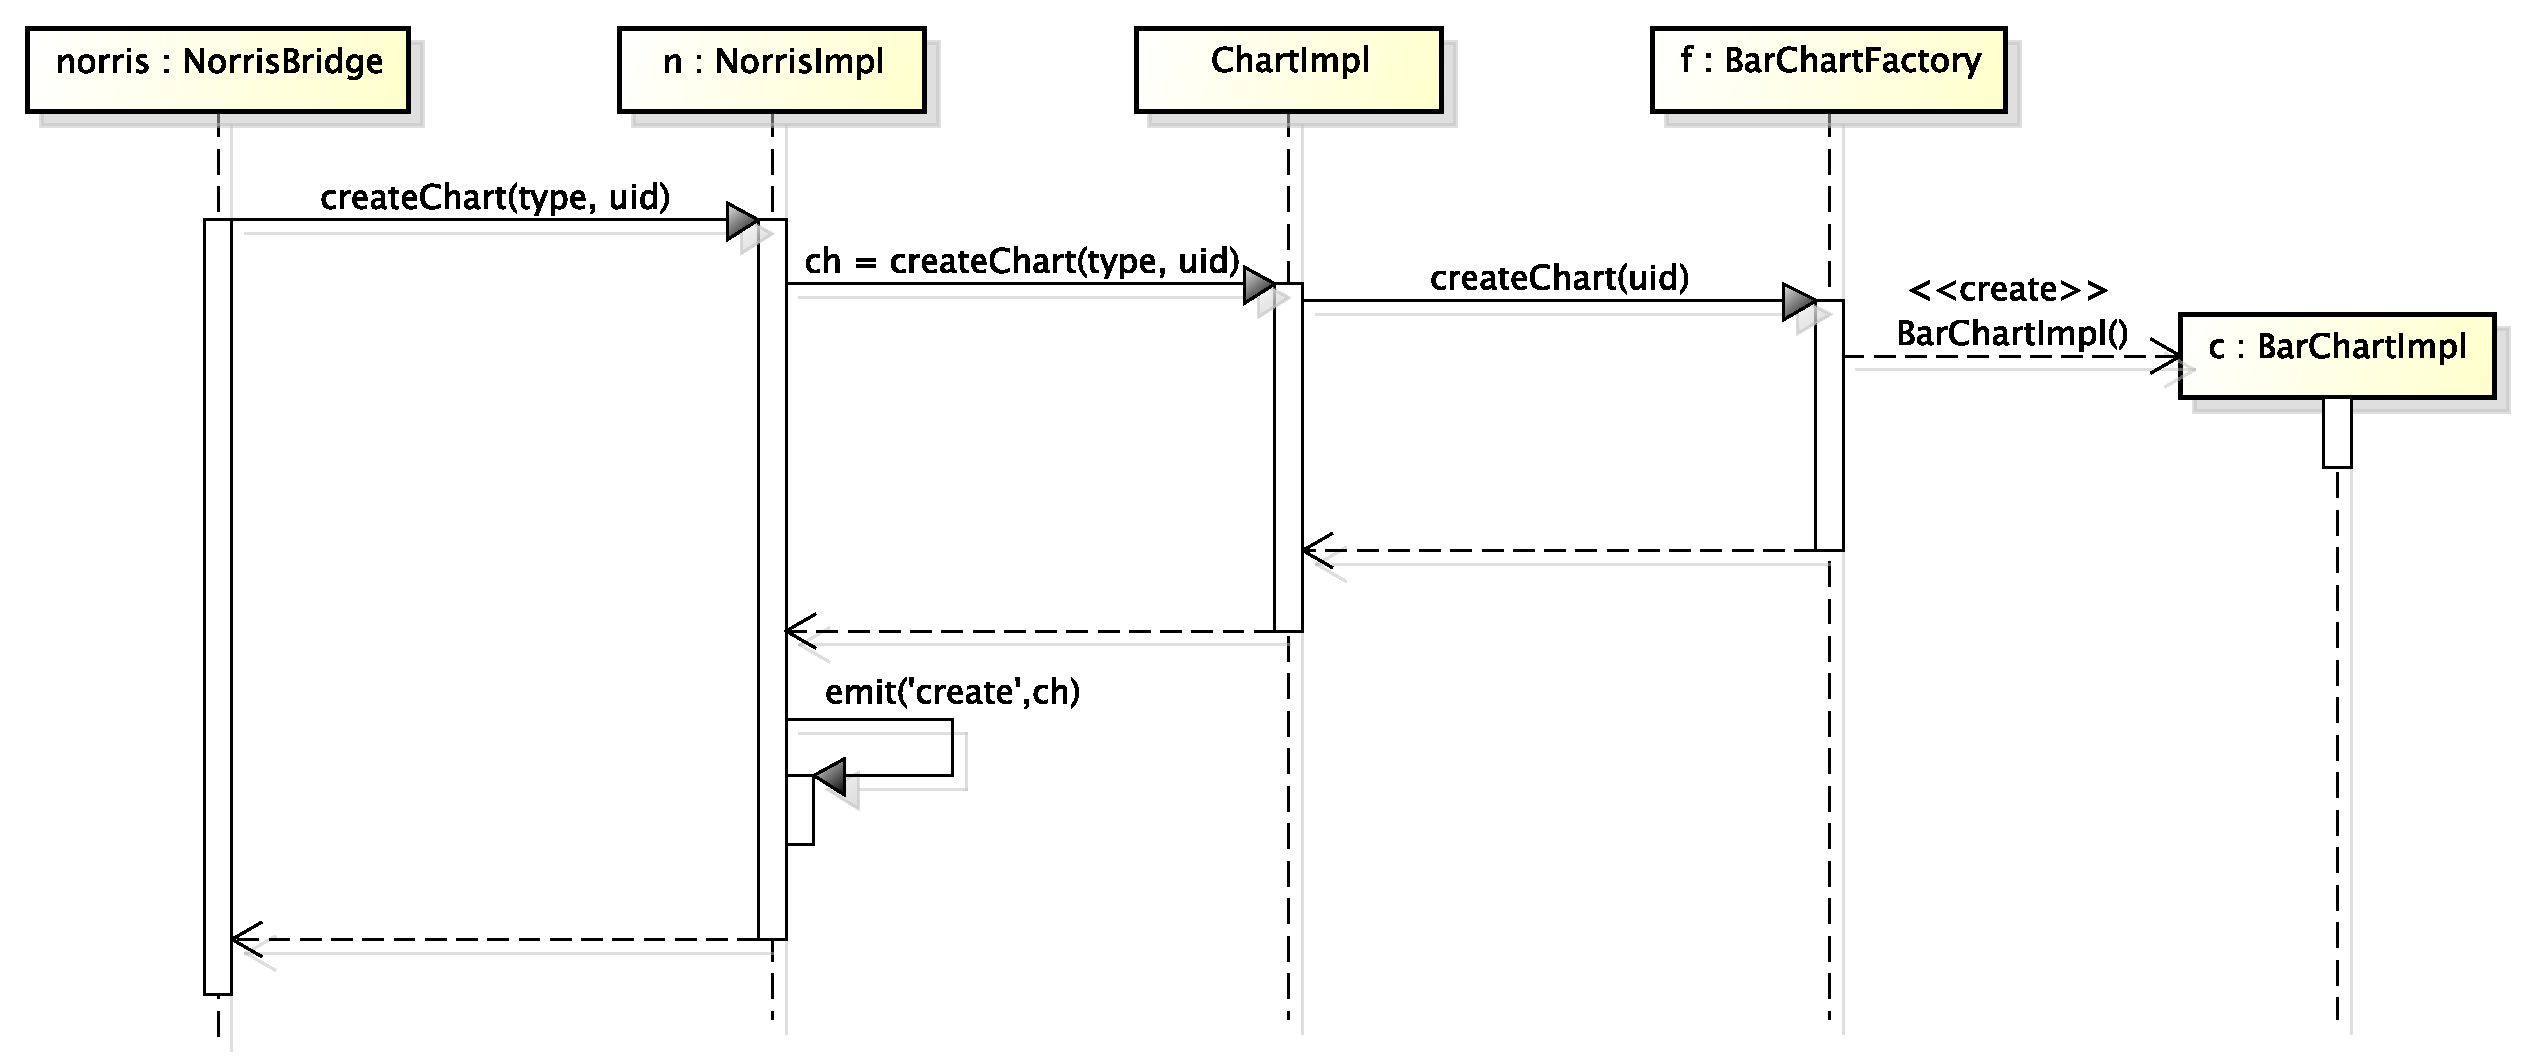
\includegraphics[scale=0.3]{DefinizioneDiProdotto/Pics/NorrisCreazioneChart}
                \caption{Diagramma di sequenza - Norris, creazione chart}
            \end{figure}
            \begin{enumerate}
                \item NorrisBridge invoca il metodo createChart di NorrisImpl in seguito all'utilizzo dell'API interna di norris per la creazione di un chart;
                \item NorrisImpl chiede la creazione del chart alla classe ChartImpl nel modello dei dati;
                \item questa crea il chart vero e proprio sfruttando la classe factory, presente all'interno dell'HashMap factories, per la creazione del chart richiesto;
                \item infine viene eseguito il metodo emit per avvertire che è avvenuta la creazione.
            \end{enumerate}


            
        \level{3}{Invio lista dei grafici}
        	Tale diagramma descrive come viene gestita la richiesta della lista di tutti i grafici contenuti in una certa istanza di \insglo{Norris}.
            \begin{figure}[H]
                \centering
                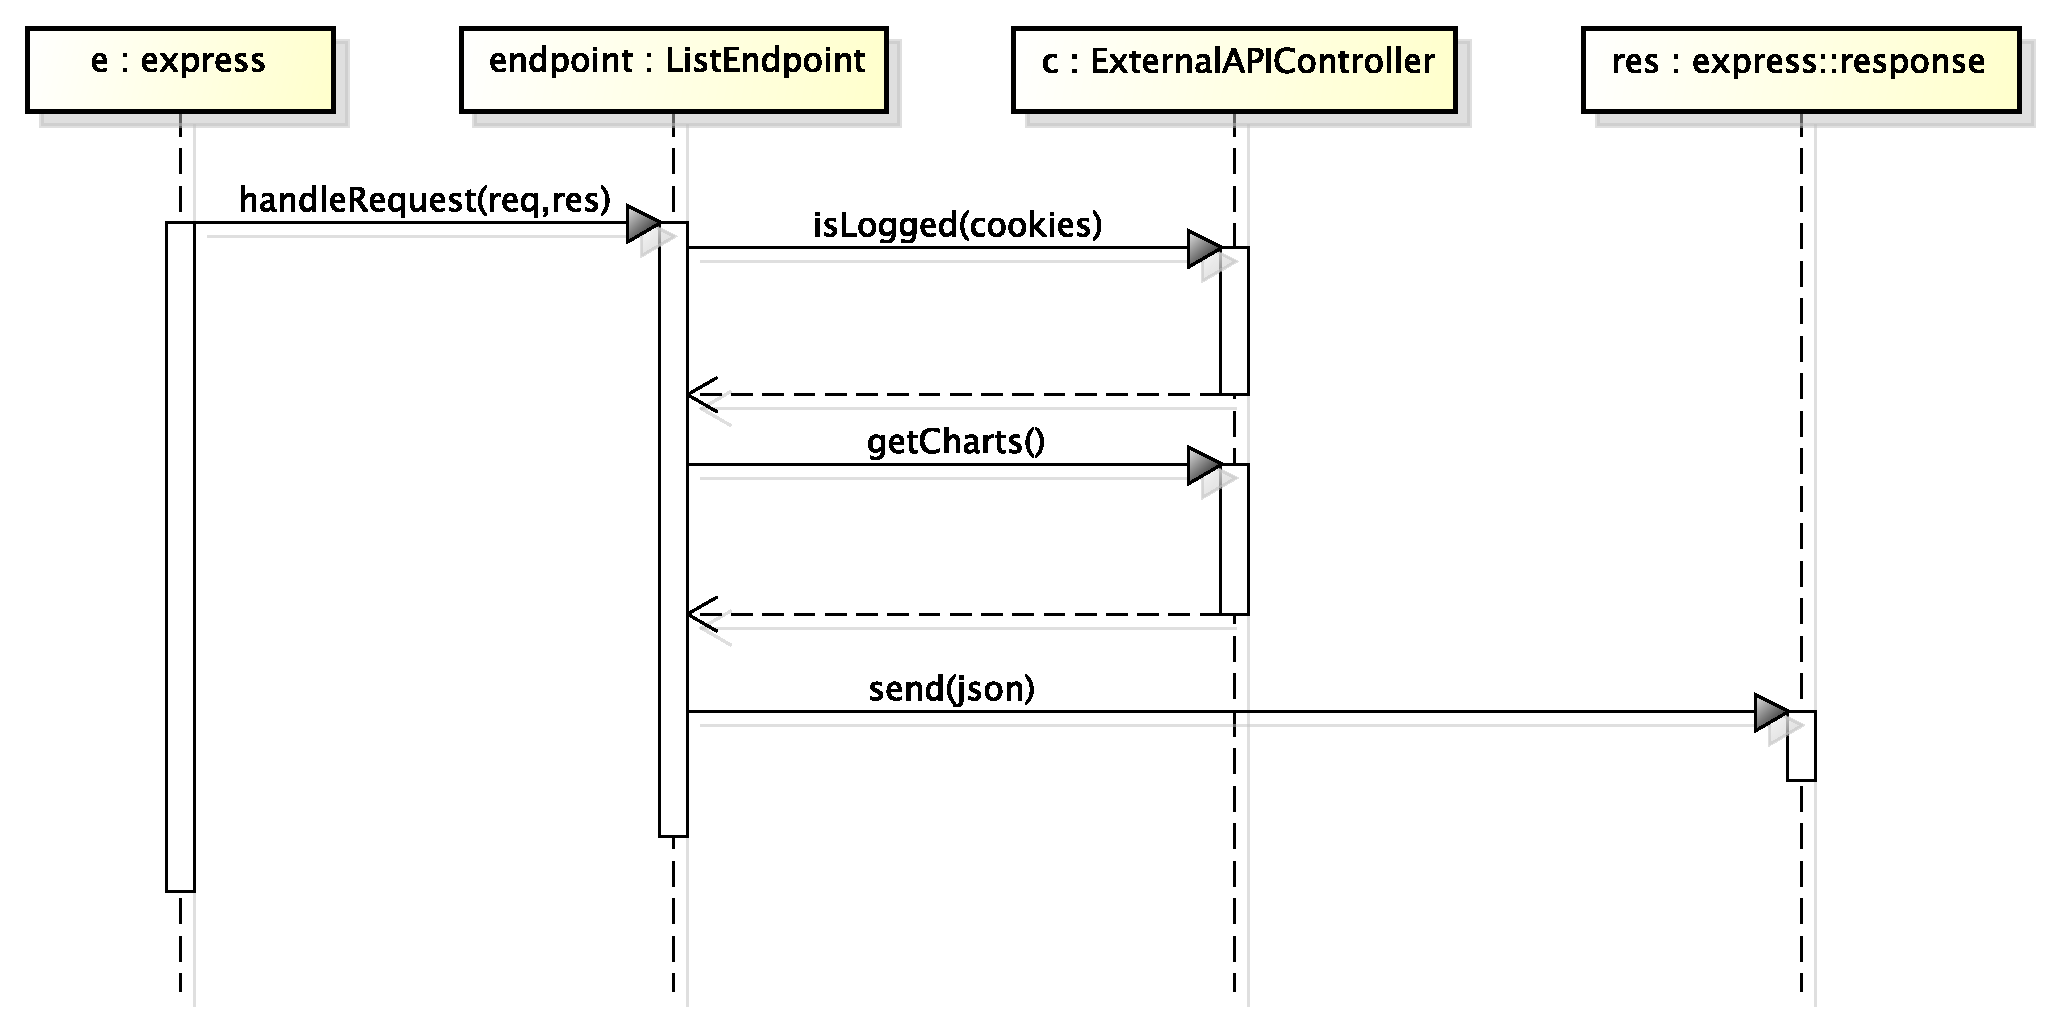
\includegraphics[scale=0.3]{DefinizioneDiProdotto/Pics/NorrisInvioLista}
                \caption{Diagramma di sequenza - Norris, invio lista}
            \end{figure}
            \begin{enumerate}
                \item alla richiesta http di tipo GET per la lista express gestisce tale richiesta dando al compito al ListEndpoint;
                \item questo controlla se la richiesta può esser soddisfatta controllando lo stato della sessione del client;
                \item ottiene la lista dei chart;
                \item infine invia la risposta con formato JSON sfruttando express.
            \end{enumerate}

            
        \level{3}{Invio di un chart}
        	Tale diagramma descrive come viene gestita la richiesta di un chart da parte di un \insglo{client} dal sistema \insglo{Norris}.
            \begin{figure}[H]
                \centering
                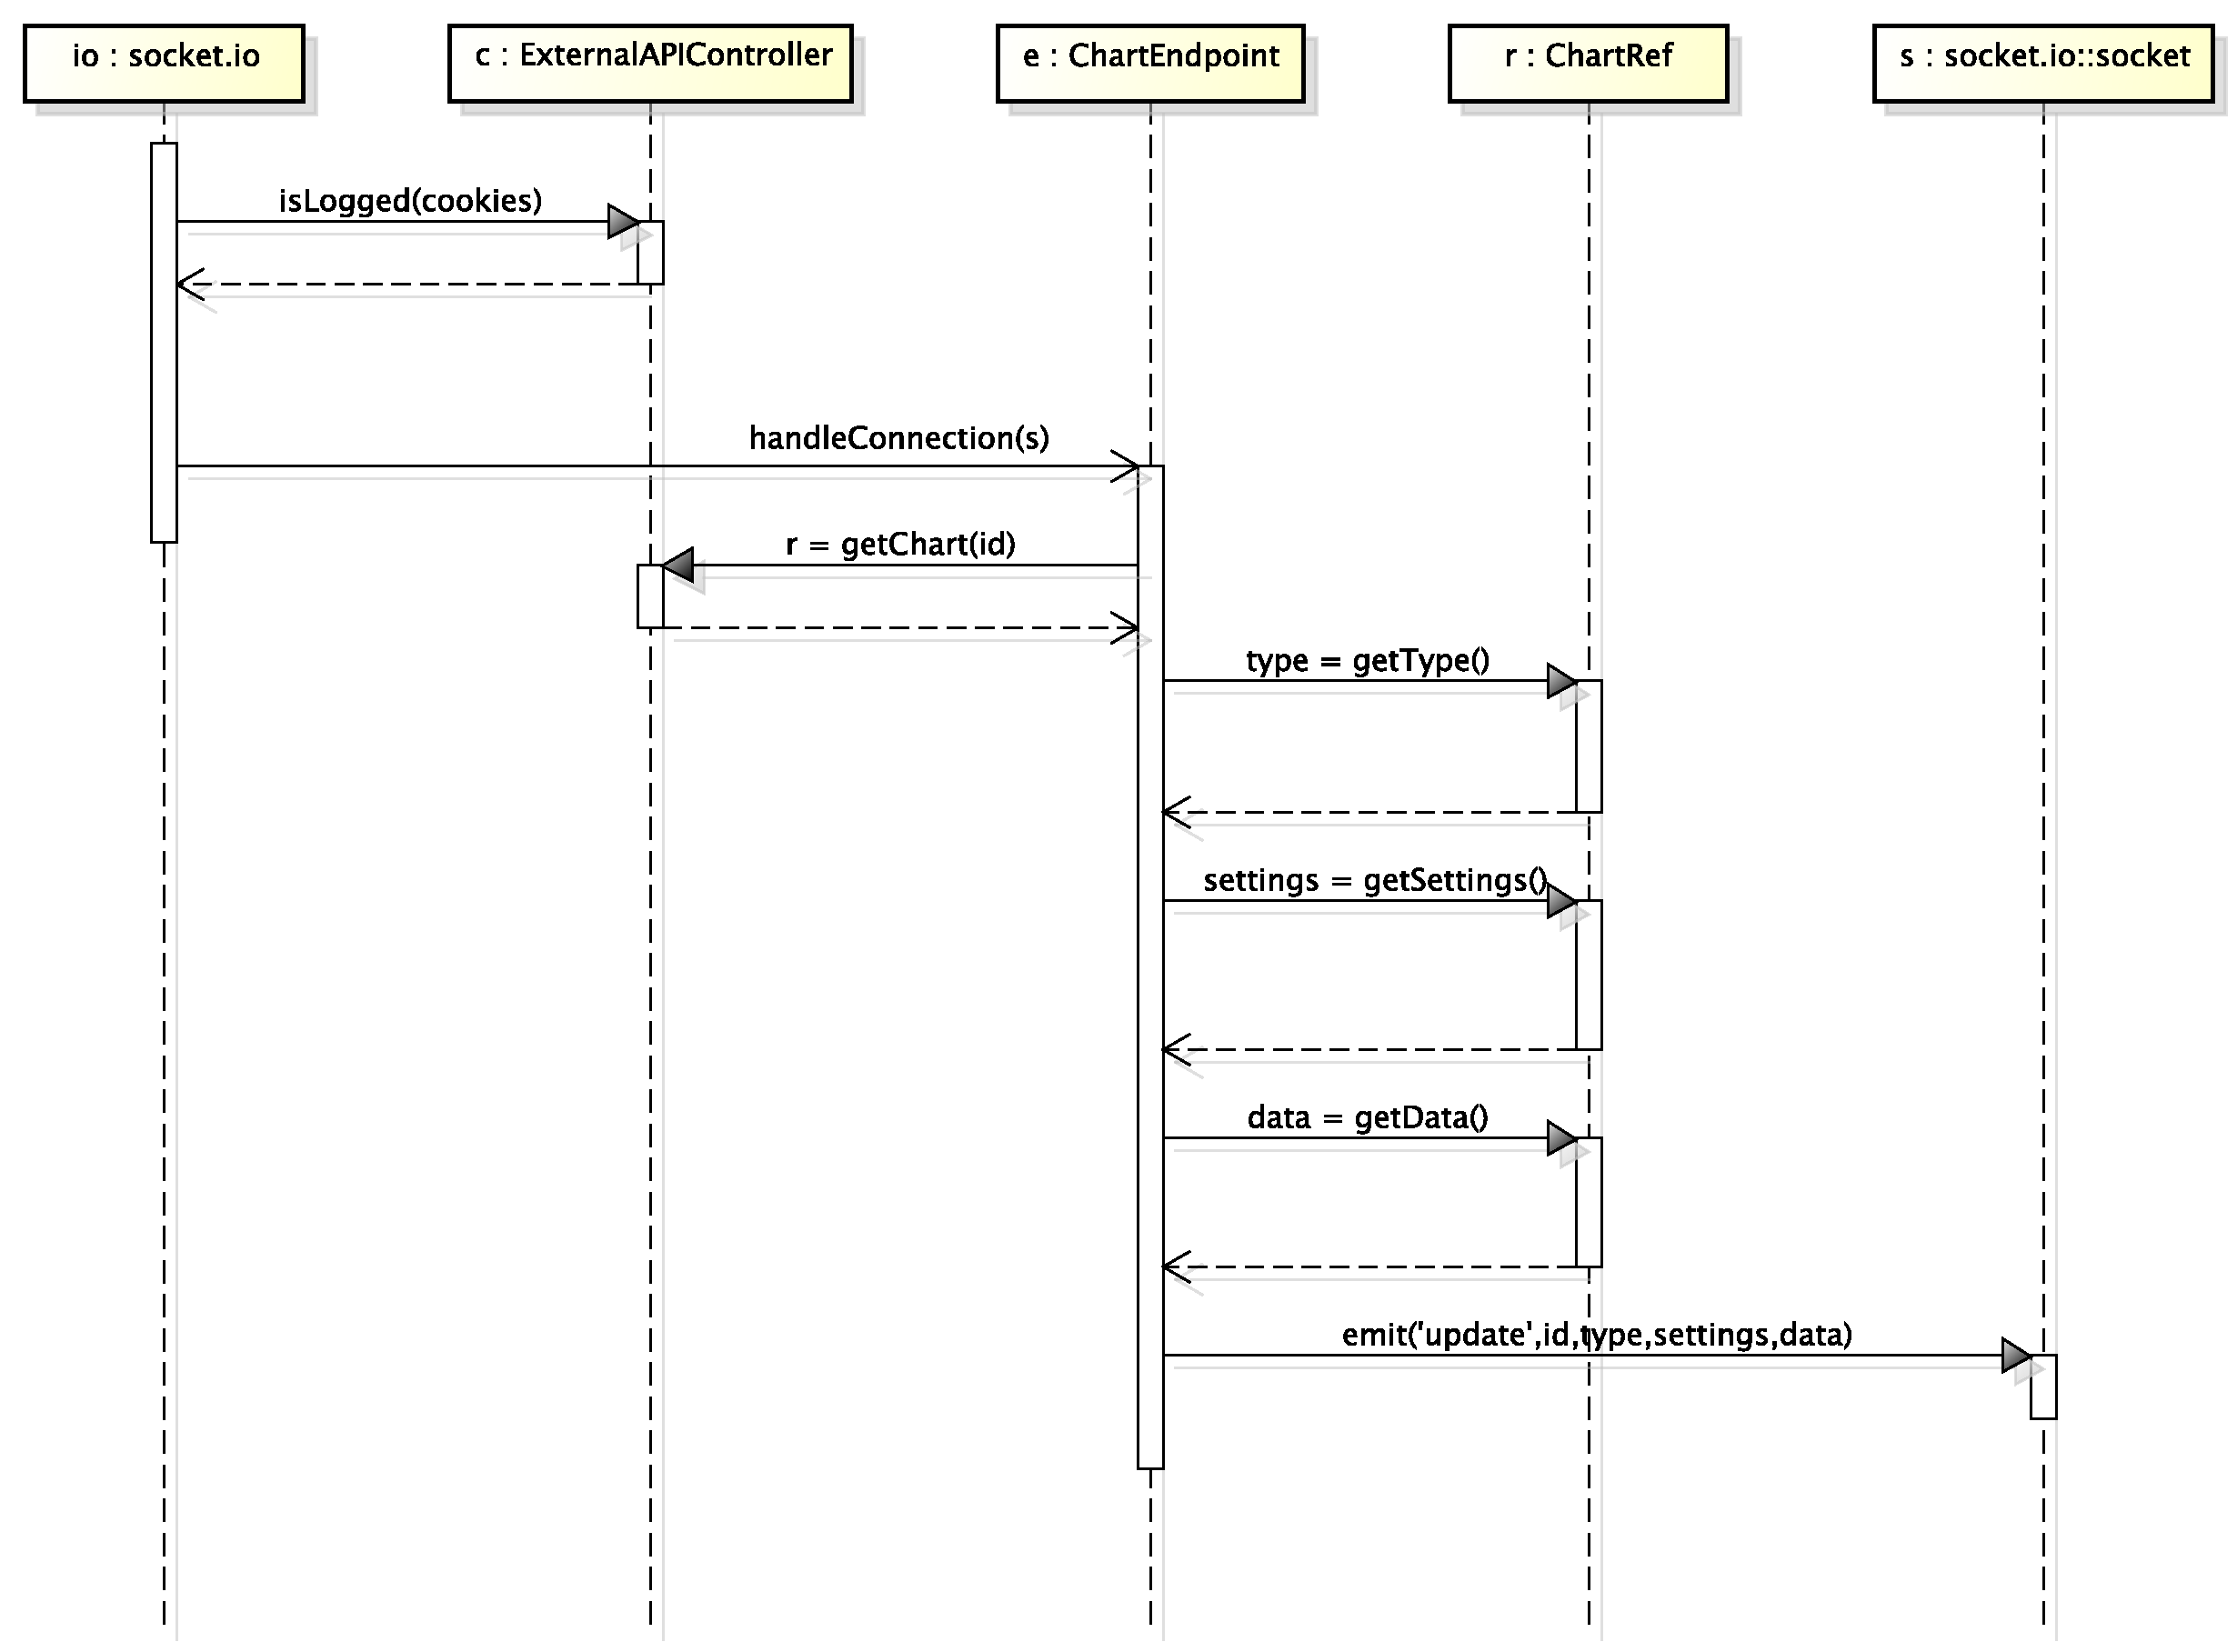
\includegraphics[scale=0.3]{DefinizioneDiProdotto/Pics/NorrisInvioChart}
                \caption{Diagramma di sequenza - Norris, invio chart}
            \end{figure}
            \begin{enumerate}
                \item la richiesta di un chart viene effettuata sfruttando il canale socket e quindi alla ricezione dell'evento di richiesta socket.io controlla se il cookie è ancora valido;
                \item viene poi dato il compito al ChartEndpoint di generare la risposta;
                \item questo ottiene il tipo del grafico;
                \item in seguito ottiene le impostazioni del grafico;
                \item l'ultima richiesta a ChartRef sono quindi i dati del grafico;
                \item infine può emettere il segnale di risposta verso il client.
            \end{enumerate}


        \level{3}{Aggiornamento di un chart}
            Tale diagramma descrive come viene aggiornato un chart di un certo tipo (sulla base delle modalità di aggiornamento definite per quel tipo di grafico).
            \begin{figure}[H]
                \centering
                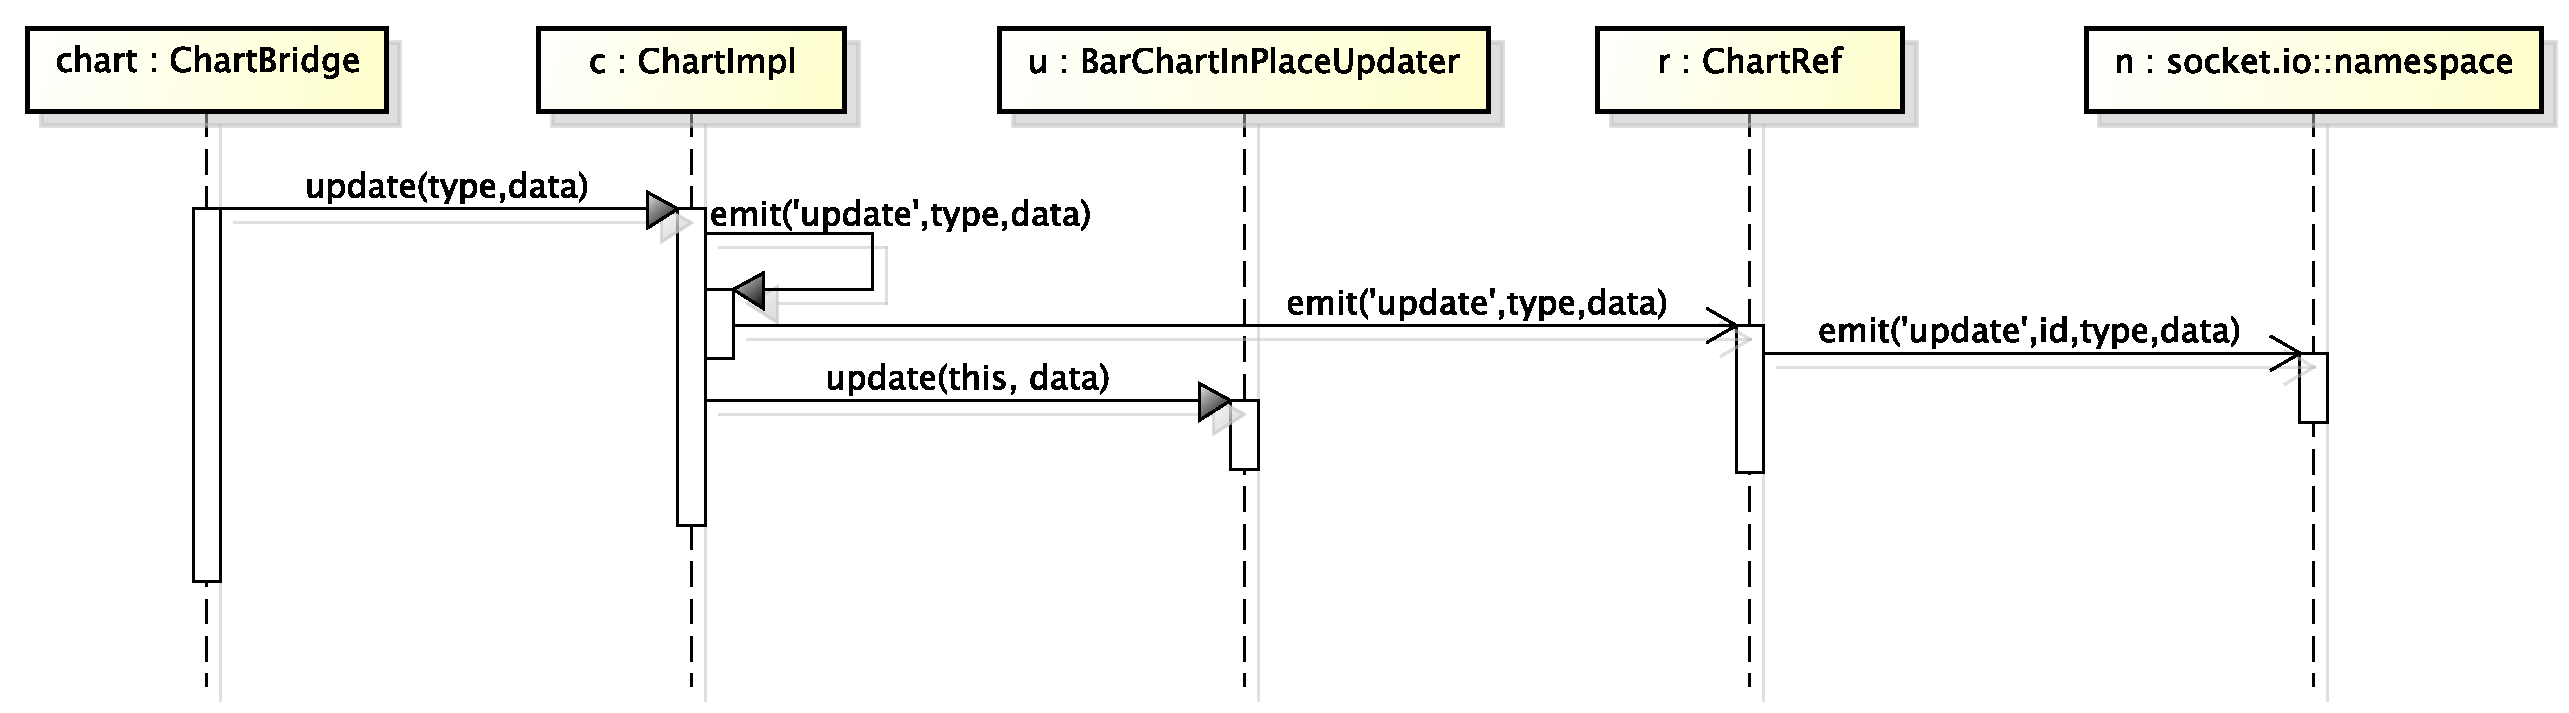
\includegraphics[scale=0.3]{DefinizioneDiProdotto/Pics/NorrisAggiornamentoChart}
                \caption{Diagramma di sequenza - Norris, aggiornamento chart}
            \end{figure}
            \begin{enumerate}
                \item all'utilizzo dell'API interna di Norris per la richiesta di aggiornamento di un chart il ChartBridge invoca il metodo di aggiorneamento nel modello dei dati (ChartImpl);
                \item questo richiederà l'aggiornamento alla classe opportuna sfruttando l'HashMap updaters;
                \item infine attraverso il canale socket vengono avvisati i vari client.
            \end{enumerate}